% rubber: setlist arguments --shell-escape

\documentclass[UKenglish,aspectratio=169]{beamer}
\usetheme[NoLogo]{pixel}


\usepackage[utf8]{inputenx} % For æ, ø, å
\usepackage{amsmath,amssymb,amsthm}

\makeatletter
\def\beamerorig@set@color{%
  \pdfliteral{\current@color}%
  \aftergroup\reset@color
}
\def\beamerorig@reset@color{\pdfliteral{\current@color}}
\makeatother


%\usepackage{babel}          % Automatic translations
%\usepackage{csquotes}       % Quotation marks
%\usepackage{microtype}      % Improved typography
%\usepackage{amssymb}        % Mathematical symbols
%\usepackage{mathtools}      % Mathematical symbols
%\usepackage[absolute, overlay]{textpos} % Arbitrary placement
%\setlength{\TPHorizModule}{\paperwidth} % Textpos units
%\setlength{\TPVertModule}{\paperheight} % Textpos units
%\usepackage{tikz}
%\usetikzlibrary{overlay-beamer-styles}  % Overlay effects for TikZ

\DeclareMathOperator*{\argmin}{arg\,min}
\DeclareMathOperator*{\argmax}{arg\,max}
\DeclareMathOperator*{\proj}{proj}
\DeclareMathOperator{\Span}{span}
\DeclareMathOperator{\Div}{div}

\usepackage{fancyvrb}
\usepackage{minted}

\definecolor{brickred}{rgb}{.79, 0.25, 0.32}
\definecolor{grass}{rgb}{.15, 0.60, 0.22}
\definecolor{postit}{rgb}{.35, 0.80, 0.99}


\author[Dmitry Sokolov]{\underline{Dmitry Sokolov}, Nicolas Ray, Étienne Corman}

\title{Least squares for programmers}
\subtitle{--- with color plates ---\\
~\\
\url{https://github.com/ssloy/least-squares-course}
}


\newcommand{\highlight}[1]{\colorbox{cyan!50}{$\displaystyle#1$}}
\newcommand\unknown[1]{\textcolor{brickred}{#1}}
\newcommand\known[1]{\textcolor{grass}{#1}}


\AtBeginSection[]
{
    \begin{frame}%[noframenumbering]
        \frametitle{Table of Contents}
        \tableofcontents[currentsection]
    \end{frame}
}

\begin{document}

%\iffalse 

%\section{Overview}
%% Use
%%
%%     \begin{frame}[allowframebreaks]{Title}
%%
%% if the TOC does not fit one frame.
%\begin{frame}{Table of contents}
%    \tableofcontents[currentsection]
%\end{frame}
%\iffalse

\begin{frame}{The goal}

This course is intended for students/engineers/researchers who know how to program in the traditional way:
by breaking down complex tasks into a sequence of elementary operations over data structures.

\vspace{2ex}

\begin{block}{An alternative}
We can describe what a good result looks like, and let numerical optimization algorithms find it for us.
\end{block}

\vspace{2ex}

This course does not require an advanced mathematical background: basic calculus knowledge suffices. A solid programming basis would be of a great aid.
\end{frame}



\section{Maximum likelihood through examples}
\begin{frame}{Coin toss experiment}
We conduct $n$ experiments, two events can happen in each one (``success'' or ``failure''):
one happens with probability $p$, the other one with probability $1-p$.

\pause
\begin{block}{The probability of getting exactly $k$ successes in these $n$ experiments}
$$
P(k;n,p) = C_n^k p^k (1-p)^{n-k}
$$
\end{block}

\pause
Toss a coin ten times ($n=10$), count the number of tails:
\begin{minipage}{.45\linewidth}
\centering
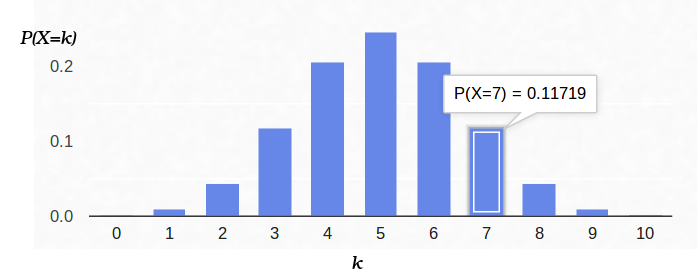
\includegraphics[width=\columnwidth]{../manuscript/img/binomial-05.png}
an ordinary coin ($p=1/2$)
\end{minipage}
\pause
\begin{minipage}{.45\linewidth}
\centering
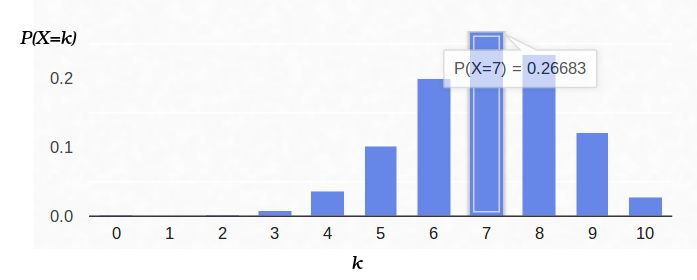
\includegraphics[width=\columnwidth]{../manuscript/img/binomial-07.png}
a biased coin ($p=7/10$)
\end{minipage}
\end{frame}

\begin{frame}{Coin toss: the likelihood function}
Suppose we have a real coin, but we do not know $p$.
However, we can toss it ten times. For example, we have counted seven tails.
Would it help us to evaluate $p$?

\pause
~\\
Fix $n=10$ and $k=7$ in Bernoulli's formula, leaving $p$ as a free parameter:
$$\mathcal{L}(\unknown{p}) = C_{\known{10}}^{\known{7}} \unknown{p}^{\known{7}} (1-\unknown{p})^{\known{3}}$$

\pause
\begin{center}
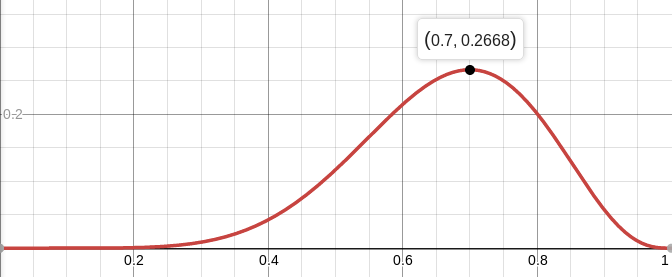
\includegraphics[width=.5\columnwidth]{../manuscript/img/likehood-07.png}
\end{center}
\textbf{N.B.} the function is continuous!
\end{frame}

\begin{frame}{Coin toss: the maximum likelihood}
Let us solve for $\argmax\limits_{\unknown{p}} \mathcal L(\unknown{p}) = \argmax\limits_{\unknown{p}} \log\mathcal{L}(\unknown{p})$:
\pause
$$\log \mathcal{L}(\unknown{p}) = \log C_{10}^7 + 7 \log \unknown{p} + 3\log (1-\unknown{p})$$
\pause
$$\frac{d \log \mathcal{L}}{d\unknown{p}} = \frac{7}{\unknown{p}} - \frac{3}{1-\unknown{p}} = 0$$

\pause
That is, the maximum likelihood (about 27\%) is reached at the point $p=7/10$.

\pause
Just in case, let us check the second derivative:
$$\frac{d^2 \log \mathcal{L}}{dp^2} = -\frac{7}{p^2} - \frac{3}{(1-p)^2}$$

At the point $p=7/10$ it is negative, therefore this point is indeed a maximum of the function $\mathcal{L}$:
$$\frac{d^2 \log \mathcal{L}}{dp^2}(0.7)  \approx -48 < 0$$
\end{frame}

\begin{frame}{Least squares through maximum likelihood}
Let us measure a constant value; all measurements are inherently noisy.

~\\

For example, if we measure the battery voltage $N$ times, we get $N$ different measurements:
$$
\{U_j\}_{j=1}^{N}
$$

Suppose that each measurement $U_j$ is i.i.d. and subject to a Gaussian noise, e.g. it is equal to the real value plus the Gaussian noise.
%The noise is characterized by two parameters --- the center of the Gaussian bell and its ``width''.
The probability density can be expressed as follows:
$$
p(U_j) = \frac{1}{\sqrt{2\pi}\unknown{\sigma}} \exp\left(-\frac{(\known{U_j}-\unknown{U})^2}{2\unknown{\sigma}^2}\right),
$$
where $U$ is the (unknown) value and $\sigma$ is the noise amplitude (can be unknown).
\end{frame}

\begin{frame}{Least squares through maximum likelihood}
$
\begin{aligned}
\log \mathcal{L}(\unknown{U},\unknown{\sigma}) & = \log \left(\prod\limits_{j=1}^N  \frac{1}{\sqrt{2\pi}\unknown{\sigma}} \exp\left(-\frac{(\known{U_j}-\unknown{U})^2}{2\unknown{\sigma}^2}\right)\right) \\ \pause
& = \sum\limits_{j=1}^N \log \left(\frac{1}{\sqrt{2\pi}\unknown{\sigma}} \exp\left(-\frac{(\known{U_j}-\unknown{U})^2}{2\unknown{\sigma}^2}\right)\right) =  \pause
  \sum\limits_{j=1}^N \left(\log \left(\frac{1}{\sqrt{2\pi}\unknown{\sigma}}\right) -\frac{(\known{U_j}-\unknown{U})^2}{2\unknown{\sigma}^2}\right)  \\ \pause
& = \underbrace{-N \left(\log\sqrt{2\pi} + \log\unknown{\sigma}\right)}_{\text{does not depend on } \{U_j\}_{j=1}^{N}} - \frac{1}{2\unknown{\sigma}^2} \sum\limits_{j=1}^N (\known{U_j}-\unknown{U})^2
\end{aligned}
$

\begin{block}{Under Gaussian noise}
\centerline{$
\argmax\limits_{\unknown{U}} \log \mathcal{L} = \argmin\limits_{\unknown{U}} \sum\limits_{j=1}^N (\known{U_j}-\unknown{U})^2
$}
\end{block}
\end{frame}

\begin{frame}{Least squares through maximum likelihood}
$
\frac{\partial\log\mathcal{L}}{\partial \unknown{U}}    = - \frac{1}{\unknown{\sigma}^2}\sum\limits_{j=1}^N (\known{U_j}-\unknown{U}) = 0 
$\\ \pause
The most plausible estimation of the unknown value $U$ is the simple average of all measurements:
$$
U = \frac{\sum\limits_{j=1}^N U_j}{N}
$$

\pause And the most plausible estimation of $\sigma$ turns out to be the standard deviation:
\begin{minipage}{.45\linewidth}
$$
\frac{\partial\log\mathcal{L}}{\partial\unknown{\sigma}} =  -\frac{N}{\unknown{\sigma}} + \frac{1}{\unknown{\sigma}^3}\sum\limits_{j=1}^N (\known{U_j}-\unknown{U})^2 = 0
$$
\end{minipage} \pause
\begin{minipage}{.45\linewidth}
$$
\sigma = \sqrt{\frac{\sum\limits_{j=1}^N (U_j-U)^2}{N}}
$$
\end{minipage}

\vspace{15pt}
Such a convoluted way to obtain a simple average of all measurements\dots
\end{frame}

\begin{frame}{Linear regression}
It is much harder for less trivial examples. Suppose we have $N$ measurements $\{x_j, y_j\}_{j=1}^{N}$,
and we want to fit a straight line onto it.

\pause
\begin{align*}
\log \mathcal{L}(\unknown{a}, \unknown{b},\unknown{\sigma}) & = \log \left(\prod\limits_{j=1}^N  \frac{1}{\sqrt{2\pi}\unknown{\sigma}} \exp\left(-\frac{(\known{y_j} - \unknown{a}\known{ x_j} - \unknown{b})^2}{2\sigma^2}\right)\right) =\\
& = \underbrace{-N \left(\log\sqrt{2\pi} + \log\unknown{\sigma}\right)}_{\text{does not depend on } \unknown{a}, \unknown{b}} - \frac{1}{2\unknown{\sigma}^2} \underbrace{\sum\limits_{j=1}^N (\known{y_j}- \unknown{a}\known{ x_j} - \unknown{b})^2}_{:=S(\unknown{a},\unknown{b})}
\end{align*}

\pause
As before,
$\argmax\limits_{\unknown{a},\unknown{b}}\log\mathcal L = \argmin\limits_{\unknown{a},\unknown{b}} S(\unknown{a}, \unknown{b})$.
\end{frame}

\begin{frame}{Linear regression}
\begin{minipage}{.45\linewidth}
$S(\unknown{a},\unknown{b}) := \sum\limits_{j=1}^N (\known{y_j}- \unknown{a}\known{ x_j} - \unknown{b})^2$
\pause
\begin{align*}
\frac{\partial S}{\partial\unknown{a}} &= \sum\limits_{j=1}^N 2 \known{x_j} (\unknown{a} \known{x_j} + \unknown{b} - \known{y_j}) = 0 \\
\frac{\partial S}{\partial\unknown{b}} &= \sum\limits_{j=1}^N 2 (\unknown{a}\known{ x_j} + \unknown{b} - \known{y_j}) = 0
\end{align*}
\end{minipage}
\begin{minipage}{.45\linewidth}
\centering
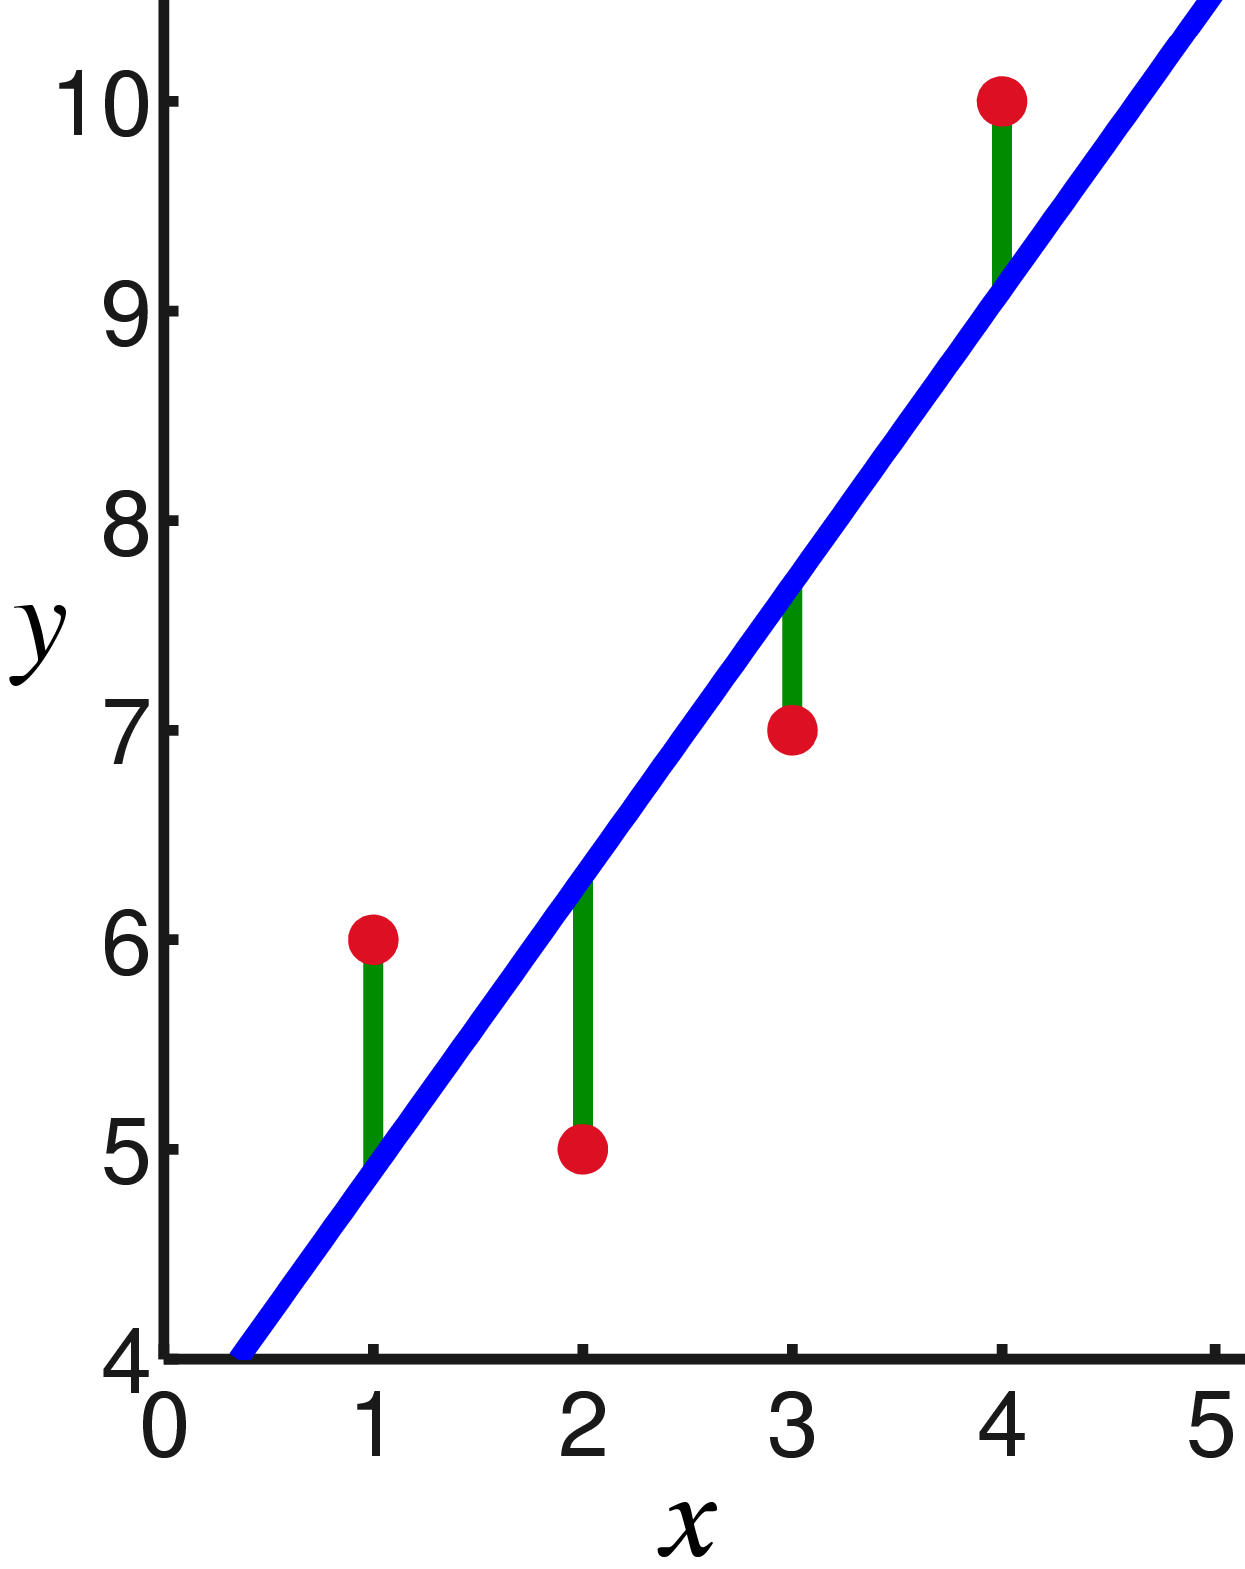
\includegraphics[width=.5\columnwidth]{../manuscript/img/c5aa80f6a2e9575abfa7b3dfdabf5c5a.png}
\end{minipage}

\pause
\begin{minipage}{.45\linewidth}
$$
a = \frac{N \sum\limits_{j=1}^N x_j y_j - \sum\limits_{j=1}^N x_j \sum\limits_{j=1}^N y_j}{N\sum\limits_{j=1}^N x_j^2 - \left(\sum\limits_{j=1}^N x_j\right)^2} \\
$$
\end{minipage}
\begin{minipage}{.45\linewidth}
$$
b = \frac{1}{N}\left(  \sum\limits_{j=1}^N y_j - a  \sum\limits_{j=1}^N x_j \right)
$$
\end{minipage}
\end{frame}

\begin{frame}{The takeaway message}
\vspace{15pt}
The least squares method is a particular case of maximizing likelihood in cases where the probability density is Gaussian.

\vspace{15pt}

The more we parameters we have, the more cumbersome the analytical solutions are.
Fortunately, we are not living in XVIII century anymore, we have computers!

\vspace{15pt}

Next we will try to build a geometric intuition on least squares, and see how can least squares problems be efficiently implemented.
\end{frame}


\section{Introduction to systems of linear equations}

\begin{frame}[fragile]{Smooth an array}
\inputminted[frame=single]{python}{listings/example_3.1.py}
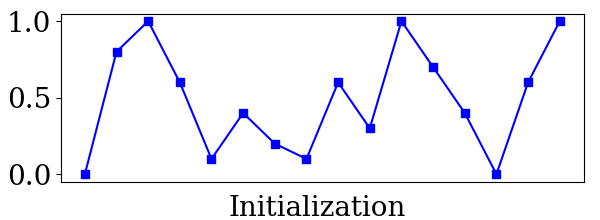
\includegraphics[width=.32\linewidth]{../manuscript/img/example_3_1_0.png}
\pause
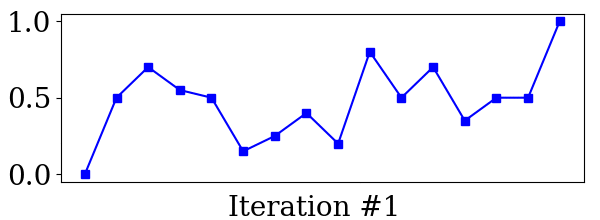
\includegraphics[width=.32\linewidth]{../manuscript/img/example_3_1_1.png}
\pause                                
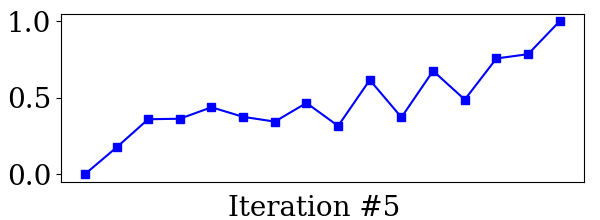
\includegraphics[width=.32\linewidth]{../manuscript/img/example_3_1_2.png}
\pause                                
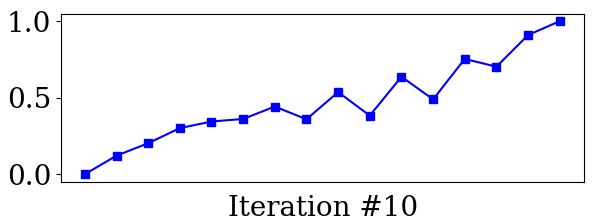
\includegraphics[width=.32\linewidth]{../manuscript/img/example_3_1_3.png}
\pause                                
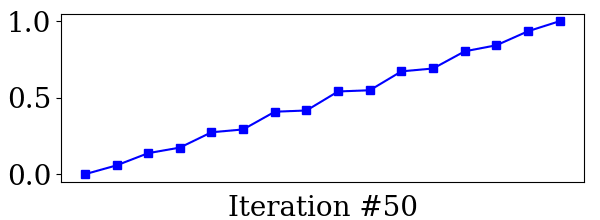
\includegraphics[width=.32\linewidth]{../manuscript/img/example_3_1_4.png}
\pause                                
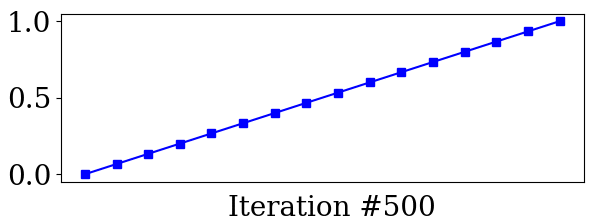
\includegraphics[width=.32\linewidth]{../manuscript/img/example_3_1_5.png}
\end{frame}

\begin{frame}{The Jacobi iterative method}
Given an ordinary system of linear equations:
%$$
%\left\{
%\begin{array}{cccccccc}
%a_{11}x_1 & + &  a_{12}x_2  &+      & \cdots & + & a_{1n}x_n &= b_1\\
%a_{21}x_1 & + &  a_{22}x_2  &+      & \cdots & + & a_{2n}x_n &= b_2\\
%          &   &             &\vdots &        &   &           &     \\
%a_{n1}x_1 & + &  a_{n2}x_2  &+      & \cdots & + & a_{nn}x_n &= b_n\\
%\end{array}
%\right.
%$$
$$
\left\{
\begin{array}{cccccccc}
\known{a_{11}}\unknown{x_1} & + &  \known{a_{12}}\unknown{x_2}  &+      & \cdots & + & \known{a_{1n}}\unknown{x_n} &= \known{b_1}\\
\known{a_{21}}\unknown{x_1} & + &  \known{a_{22}}\unknown{x_2}  &+      & \cdots & + & \known{a_{2n}}\unknown{x_n} &= \known{b_2}\\
          &   &             &\vdots &        &   &           &     \\
\known{a_{n1}}\unknown{x_1} & + &  \known{a_{n2}}\unknown{x_2}  &+      & \cdots & + & \known{a_{nn}}\unknown{x_n}&= \known{b_n}\\
\end{array}
\right.
$$


\pause
Let us rewrite it as follows:
\begin{align*}
\unknown{x_1} &= \frac{1}{\known{a_{11}}}(\known{b_1} - \known{a_{12}}\unknown{x_2} - \known{a_{13}}\unknown{x_3} - \cdots - \known{a_{1n}}\unknown{x_n})\\
\unknown{x_2} &= \frac{1}{\known{a_{22}}}(\known{b_2} - \known{a_{21}}\unknown{x_1} - \known{a_{23}}\unknown{x_3} - \cdots - \known{a_{2n}}\unknown{x_n})\\
    & \qquad \vdots \\
\unknown{x_n} &= \frac{1}{\known{a_{nn}}}(\known{b_n} - \known{a_{n1}}\unknown{x_1} - \known{a_{n2}}\unknown{x_2} - \cdots - \known{a_{n,n-1}}\unknown{x_{n-1}})
\end{align*}
%Let us rewrite it as follows:
%\begin{align*}
%x_1 &= \frac{1}{a_{11}}(b_1 - a_{12}x_2 - a_{13}x_3 - \cdots - a_{1n}x_n)\\
%x_2 &= \frac{1}{a_{22}}(b_2 - a_{21}x_1 - a_{23}x_3 - \cdots - a_{2n}x_n)\\
%    & \qquad \vdots \\
%x_n &= \frac{1}{a_{nn}}(b_n - a_{n1}x_1 - a_{n2}x_2 - \cdots - a_{n,n-1}x_{n-1})
%\end{align*}
\end{frame}

\begin{frame}{The Jacobi iterative method}
Let us start with an arbitrary vector $\vec{x}^{(0)}=\left(x_1^{(0)}, x_2^{(0)}, \dots, x_n^{(0)}\right)$,\\
\pause
we can define $\vec{x}^{(1)}$ as follows:
\begin{align*}
x_1^{(1)} &= \frac{1}{\known{a_{11}}}(\known{b_1} - \known{a_{12}}x_2^{(0)} - \known{a_{13}}x_3^{(0)} - \cdots - \known{a_{1n}}x_n^{(0)})\\
x_2^{(1)} &= \frac{1}{\known{a_{22}}}(\known{b_2} - \known{a_{21}}x_1^{(0)} - \known{a_{23}}x_3^{(0)} - \cdots - \known{a_{2n}}x_n^{(0)})\\
    & \qquad \vdots \\
x_n^{(1)} &= \frac{1}{\known{a_{nn}}}(\known{b_n} - \known{a_{n1}}x_1^{(0)} - \known{a_{n2}}x_2^{(0)} - \cdots - \known{a_{n,n-1}}x_{n-1}^{(0)})
\end{align*}
%\begin{align*}
%x_1^{(1)} &= \frac{1}{a_{11}}(b_1 - a_{12}x_2^{(0)} - a_{13}x_3^{(0)} - \cdots - a_{1n}x_n^{(0)})\\
%x_2^{(1)} &= \frac{1}{a_{22}}(b_2 - a_{21}x_1^{(0)} - a_{23}x_3^{(0)} - \cdots - a_{2n}x_n^{(0)})\\
%    & \qquad \vdots \\
%x_n^{(1)} &= \frac{1}{a_{nn}}(b_n - a_{n1}x_1^{(0)} - a_{n2}x_2^{(0)} - \cdots - a_{n,n-1}x_{n-1}^{(0)})
%\end{align*}
\pause
Repeating the process $k$ times, the solution can be approximated by the vector $\vec{x}^{(k)}=\left(x_1^{(k)}, x_2^{(k)}, \dots, x_n^{(k)}\right)$.
\end{frame}

\begin{frame}{Back to the array smoothing}
\inputminted[frame=single]{python}{listings/example_3.1.py}
\pause
\begin{minipage}{.45\linewidth}
$$x_i = \frac{x_{i-1}+x_{i+1}}{2}$$
\pause 
$$\Updownarrow$$ $$ x_i-x_{i-1} = x_{i+1} - x_i$$
%\begin{minted}[linenos=false]{python}
%x[i] = (x[i-1] + x[i+1]) / 2
%\end{minted}
\end{minipage}
\pause
\begin{minipage}{.45\linewidth}
$$
\left\{
\begin{array}{rl}
 x_0 &= 0 \\
x_1-x_0 &= x_2-x_1 \\
x_2-x_1 &= x_3-x_1 \\
     &  \vdots \\
x_{13}-x_{12}     &= x_{14}-x_{13} \\
x_{14}-x_{13}     &= x_{15}-x_{14} \\
x_{15} &= 1 \\
\end{array}
\right.
$$
\end{minipage}
\end{frame}

\begin{frame}{Jacobi vs Gauß--Seidel}
\vspace{-8mm}
\begin{align*}
x_1^{(1)} &= \frac{1}{\known{a_{11}}}(\known{b_1} - \known{a_{12}}x_2^{(0)} - \known{a_{13}}x_3^{(0)} - \cdots - \known{a_{1n}}x_n^{(0)})\\
x_2^{(1)} &= \frac{1}{\known{a_{22}}}(\known{b_2} - \known{a_{21}}x_1^{(0)} - \known{a_{23}}x_3^{(0)} - \cdots - \known{a_{2n}}x_n^{(0)})\\
    & \qquad \vdots \\
\end{align*}
\pause
\begin{align*}
\highlight{x_1^{(1)}} &= \frac{1}{\known{a_{11}}}(\known{b_1} - \known{a_{12}}x_2^{(0)} - \known{a_{13}}x_3^{(0)} - \cdots - \known{a_{1n}}x_n^{(0)})\\
x_2^{(1)} &= \frac{1}{\known{a_{22}}}(\known{b_2} - \known{a_{21}}\highlight{x_1^{(1)}} - \known{a_{23}}x_3^{(0)} - \cdots - \known{a_{2n}}x_n^{(0)})\\
    & \qquad \vdots \\
\end{align*}
\end{frame}


\begin{frame}{Jacobi vs Gauß--Seidel}
Jacobi:
$$
x_i^{(k)} = \frac{1}{a_{ii}} \left(b_i - \sum\limits_{j=1,j\neq i}^n a_{ij}x_j^{(k-1)} \right), \quad \text{for } i=1,2,\dots,n
$$
\pause

\vspace{47pt}
Gauß-Seidel:
$$
x_i^{(k)} = \frac{1}{a_{ii}} \left(b_i - \sum\limits_{j=1}^{i-1} a_{ij}x_j^{(k)} -  \sum\limits_{j=i+1}^n a_{ij}x_j^{(k-1)} \right), \quad \text{for } i=1,2,\dots,n
$$
\end{frame}

\begin{frame}{Jacobi vs Gauß--Seidel}
Jacobi:
\inputminted[frame=single]{python}{listings/example_3.1.py}

Gauß--Seidel:
\inputminted[frame=single]{python}{listings/example_3.2.py}
\end{frame}

\begin{frame}[fragile]{Smooth an array : Gauß--Seidel}
\inputminted[frame=single]{python}{listings/example_3.2.py}
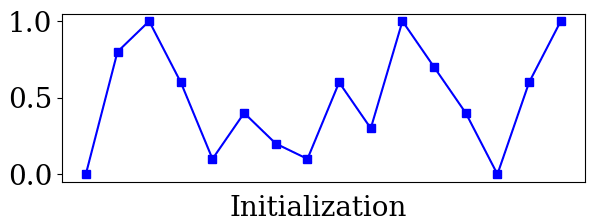
\includegraphics[width=.32\linewidth]{../manuscript/img/example_3_2_0.png}
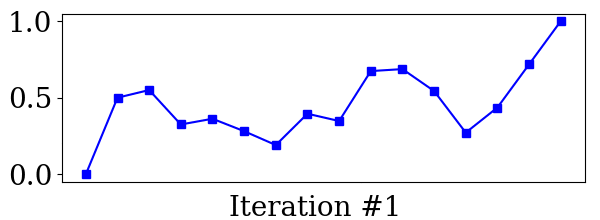
\includegraphics[width=.32\linewidth]{../manuscript/img/example_3_2_1.png}
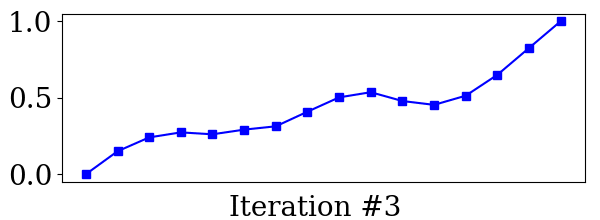
\includegraphics[width=.32\linewidth]{../manuscript/img/example_3_2_2.png}
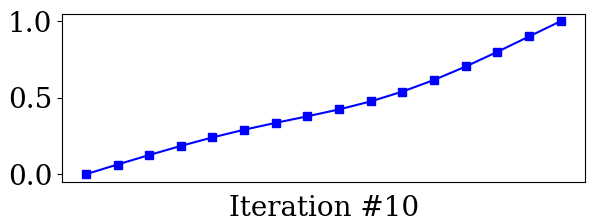
\includegraphics[width=.32\linewidth]{../manuscript/img/example_3_2_3.png}
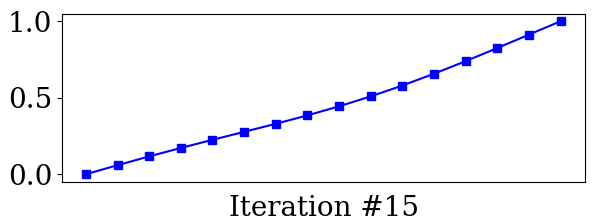
\includegraphics[width=.32\linewidth]{../manuscript/img/example_3_2_4.png}
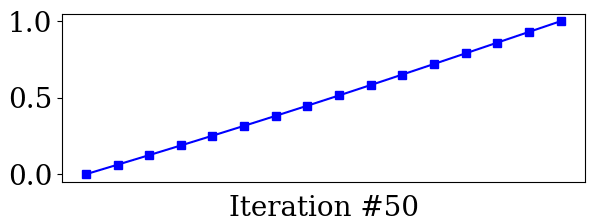
\includegraphics[width=.32\linewidth]{../manuscript/img/example_3_2_5.png}
\end{frame}


\begin{frame}{Equality of derivatives vs zero curvature}
\inputminted[frame=single]{python}{listings/example_3.2.py}
\only<1>{
$$
\left\{
\begin{array}{rl}
 x_0 &= 0 \\
x_1-x_0 &= x_2-x_1 \\
x_2-x_1 &= x_3-x_1 \\
     &  \vdots \\
x_{13}-x_{12}     &= x_{14}-x_{13} \\
x_{14}-x_{13}     &= x_{15}-x_{14} \\
x_{15} &= 1 \\
\end{array}
\right.
$$
}
\only<2>{
$$
\left\{
\begin{array}{rrrrrrrl}
 x_0 &       &       &       &        &           &         &= 0 \\
-x_0 & +2x_1 & -x_2  &       &        &           &         &= 0 \\
     &  -x_1 & +2x_2  & -x_3 &        &           &         &= 0 \\
     &       & \ddots      & \ddots & \ddots&          &         &  \vdots \\
     &       &       & -x_{12}  & +2x_{13} & -x_{14}  &         &= 0 \\
     &       &       &          & -x_{13}  & +2x_{14} & -x_{15} &= 0 \\
     &       &       &          &          &          &  x_{15} &= 1 \\
\end{array}
\right.
$$
}
\end{frame}

\begin{frame}{It also works for 3d surfaces}
\only<1>{
%\inputminted[frame=single]{cpp}{listings/example_3.3.cpp}
\inputminted[fontsize=\scriptsize,frame=single]{python}{listings/smooth-neanderthal.py}
}
\only<2>{
    \vspace{10pt}
    \begin{centering}
    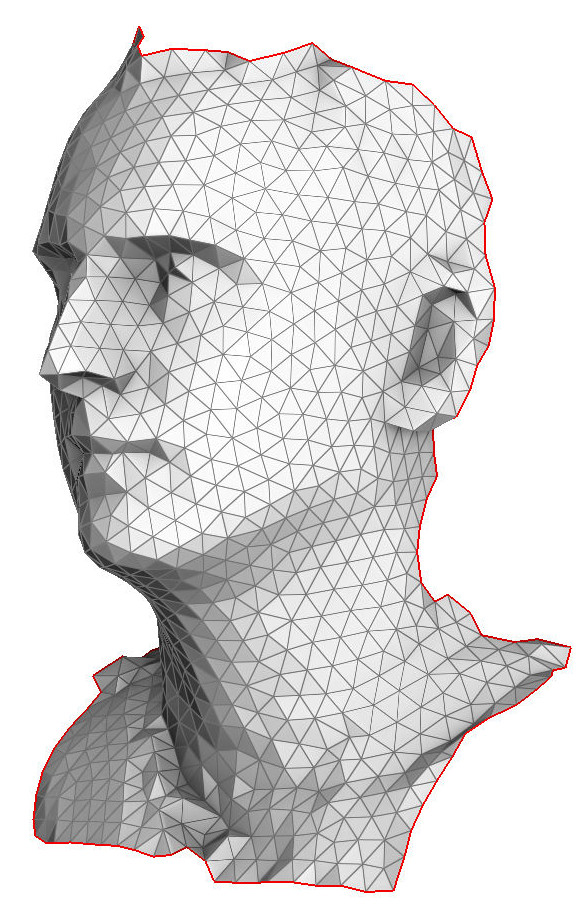
\includegraphics[width=.2\linewidth]{../manuscript/img/example_3_3_0.jpg}
    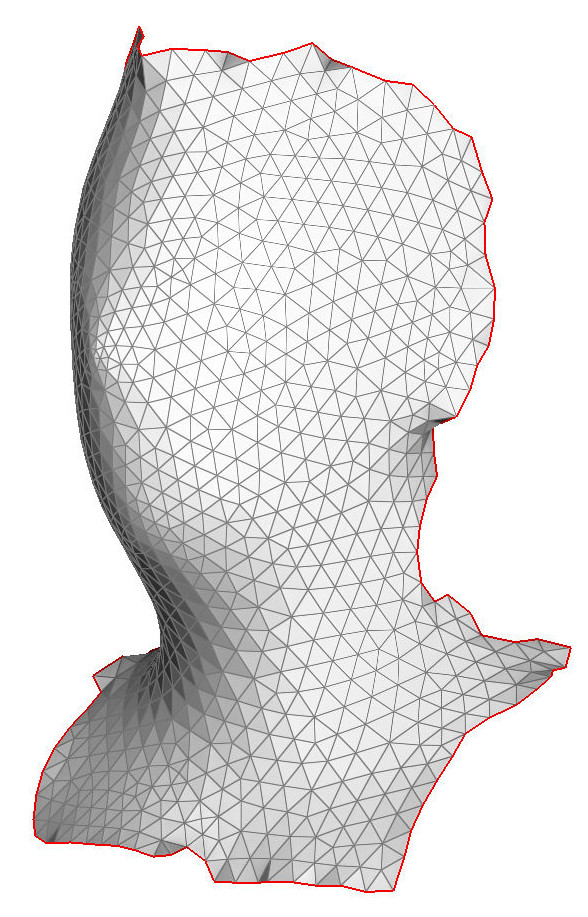
\includegraphics[width=.2\linewidth]{../manuscript/img/example_3_3_1.jpg}
    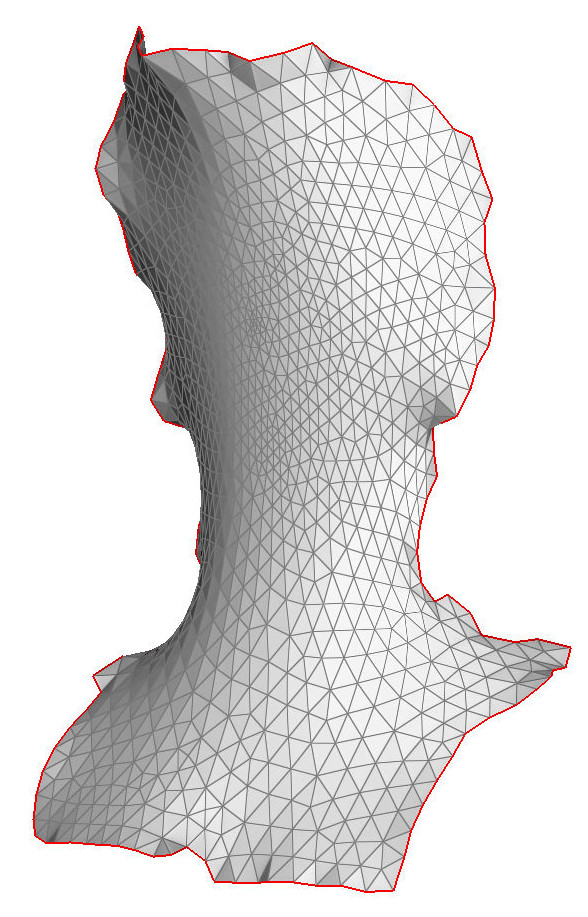
\includegraphics[width=.2\linewidth]{../manuscript/img/example_3_3_2.jpg}\\
    \hspace{.25\linewidth} input \hspace{.11\linewidth} 10 iterations \hspace{.05\linewidth} 1000 iterations
    \end{centering}
}
\end{frame}

\begin{frame}{Prescribe the right hand side}
\inputminted[frame=single]{python}{listings/example_3.4.py}
\pause
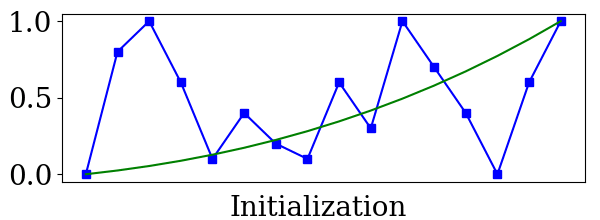
\includegraphics[width=.32\linewidth]{../manuscript/img/example_3_4_0.png}
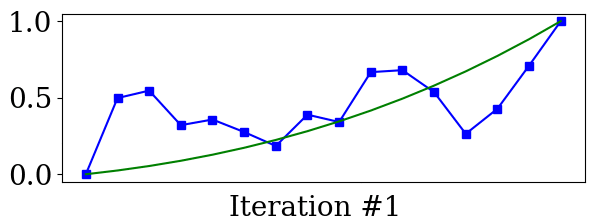
\includegraphics[width=.32\linewidth]{../manuscript/img/example_3_4_1.png}
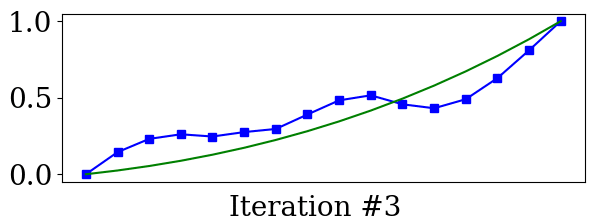
\includegraphics[width=.32\linewidth]{../manuscript/img/example_3_4_2.png}
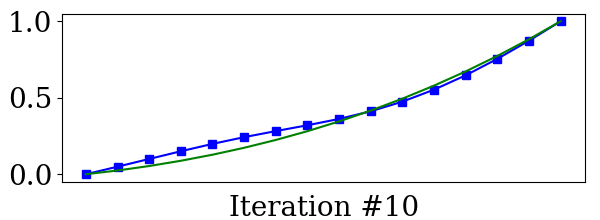
\includegraphics[width=.32\linewidth]{../manuscript/img/example_3_4_3.png}
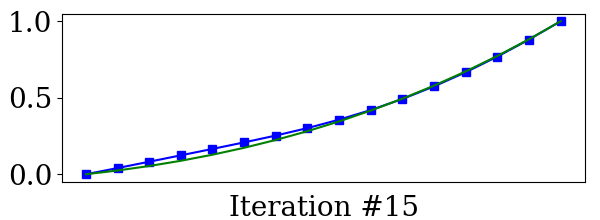
\includegraphics[width=.32\linewidth]{../manuscript/img/example_3_4_4.png}
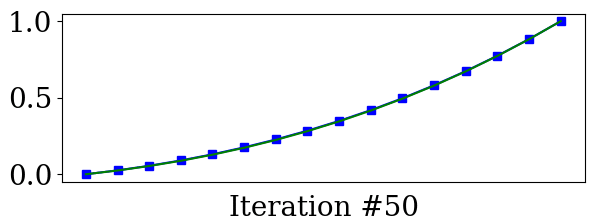
\includegraphics[width=.32\linewidth]{../manuscript/img/example_3_4_5.png}
Well duh... Of course it is a cubic polynomial!
\end{frame}



\begin{frame}{The takeaway message}

\vspace{25pt}
We just saw that mere 3 lines of code  can be sufficient to solve a linear system, 
effectively solving a differential equation.

\vspace{25pt}
While it is extremely cool, it raises questions:
\begin{itemize}
\item What are the practical consequences for a programmer?
\item How do we build these systems?
\item Where do we use them?
\end{itemize}
\end{frame}




\section{Minimization of quadratic functions}
%\SectionPage

\begin{frame}[fragile]{Matrices and numbers}
What is a number $a$?
\begin{minted}[linenos=true]{cpp}
float a = 2.7;
\end{minted}
\pause

\begin{minipage}{.5\linewidth}
Is it a function $y(x)=ax : \mathbb R \rightarrow \mathbb R$?
\pause
\begin{minted}[linenos=true]{cpp}
float y(float x) {
    return a*x;
}
\end{minted}
\end{minipage}
\begin{minipage}{.45\linewidth}

\includegraphics[width=.35\linewidth]{../manuscript/img/2_7x.png}
\end{minipage}
\pause

~\\

\begin{minipage}{.5\linewidth}
Or is it $y(x)=ax^2 : \mathbb R \rightarrow \mathbb R$?
\pause
\begin{minted}[linenos=true]{cpp}
float y(float x) {
    return x*a*x;
}
\end{minted}
\end{minipage}
\begin{minipage}{.45\linewidth}
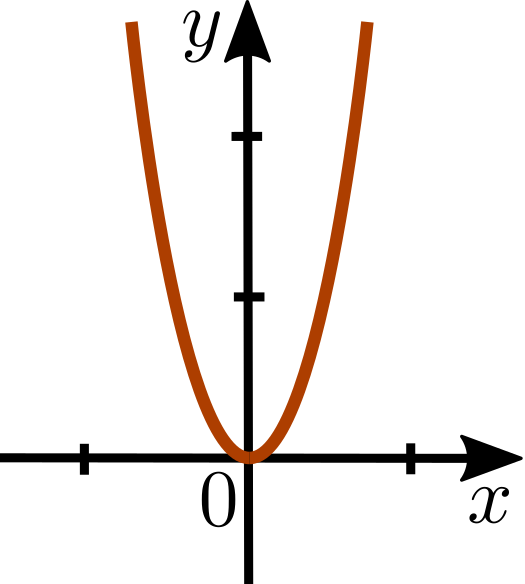
\includegraphics[width=.35\linewidth]{../manuscript/img/2_7x2.png}
\end{minipage}
\end{frame}

\begin{frame}[fragile]{Matrices and numbers}
The same goes for matrices, what is a matrix $A=\begin{bmatrix} a_{11} & a_{12} \\ a_{21} & a_{22}\end{bmatrix}$?
\pause
\begin{minted}{cpp}
float A[2][2] = {{1., .5}, {.5, 1.}};
\end{minted}

\pause
~\\
\begin{minipage}{.7\linewidth}
Is it $f(x) = Ax : \mathbb R^2 \rightarrow \mathbb R^2$?
\begin{minted}[linenos=true]{cpp}
vector<float> f(vector<float> x) {
  return vector<float>{a11*x[0] + a12*x[1],
                       a21*x[0] + a22*x[1]};
}
\end{minted}
\end{minipage}
\begin{minipage}{.28\linewidth}
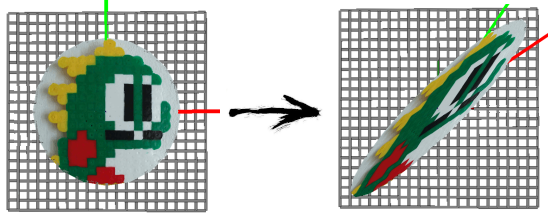
\includegraphics[width=\linewidth]{../manuscript/img/matrix-linear.png}
\end{minipage}

\pause
\begin{minipage}{.7\linewidth}
\vspace{2ex}
Or $f(x)= x^\top A x = \sum\limits_i\sum\limits_j a_{ij}x_i x_j  : \mathbb R^2 \rightarrow \mathbb R$?
\begin{minted}[linenos=true]{cpp}
float f(vector<float> x) {
    return x[0]*a11*x[0] + x[0]*a12*x[1] +
           x[1]*a21*x[0] + x[1]*a22*x[1];
}
\end{minted}
\end{minipage}
\begin{minipage}{.28\linewidth}
\centering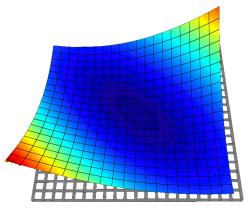
\includegraphics[width=.7\linewidth]{../manuscript/img/matrix-quadratic-form.png}
\end{minipage}
\end{frame}

\begin{frame}{What is a positive number?}
We have a great tool called the predicate ``greater than'' $>$.
\pause
\begin{definition}
The real number $a$ is positive if and only if for all non-zero real $x\in\mathbb R,\ x\neq 0$ the condition $ax^2>0$ is satisfied.
\end{definition}
\pause
~\\
This definition looks pretty awkward, but it applies perfectly to matrices:
\begin{definition}
The square matrix $A$ is called positive definite if for any non-zero $x$
the condition $x^\top A x > 0$ is met, i.e. the corresponding quadratic form is strictly positive everywhere except at the origin.
\end{definition}
\end{frame}

\begin{frame}{What is a positive number?}
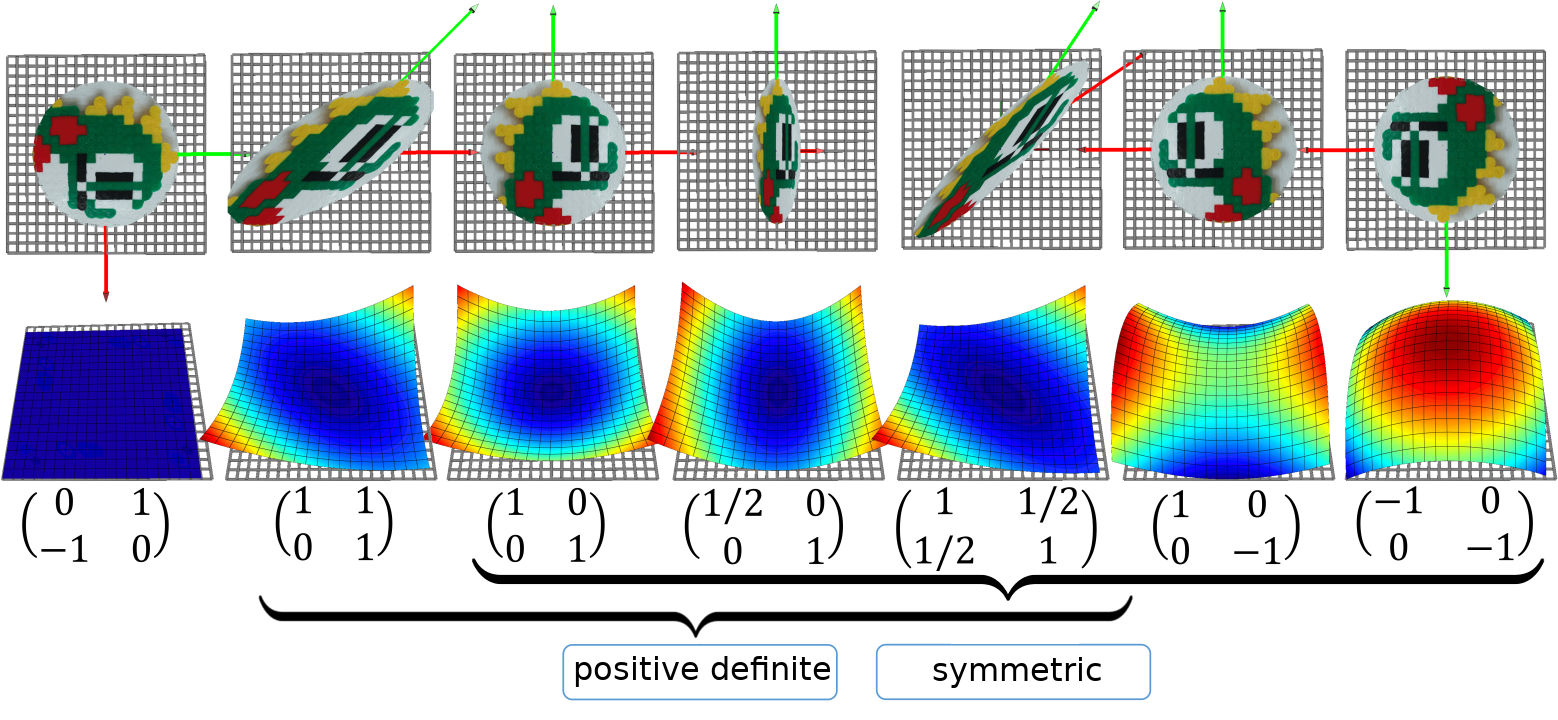
\includegraphics[width=\linewidth]{../manuscript/img/matrices}
\end{frame}

\begin{frame}{Minimizing a 1d quadratic function}
Let us find the minimum of the function $f(x) = ax^2 - 2bx$ (with $a$ positive).
$$\frac{d}{dx}f(x) = 2ax - 2b = 0$$
\pause
\begin{center}
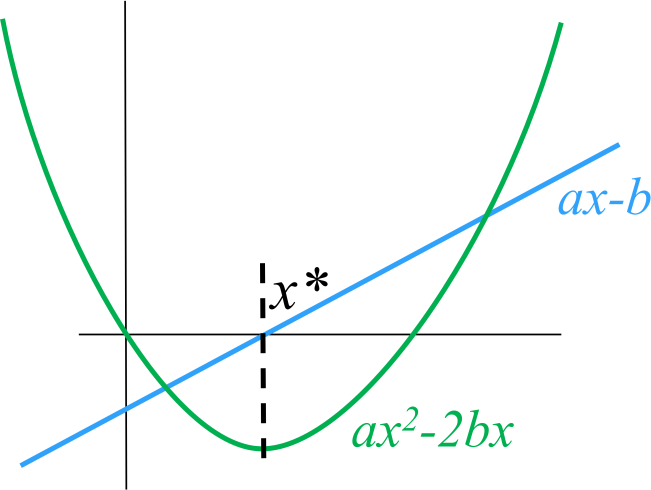
\includegraphics[width=.3\linewidth]{../manuscript/img/minpb1d}
\end{center}
In 1d, the solution $x^*$ of the equation $ax - b = 0$ solves the minimization problem $\argmin\limits_x(ax^2-2bx)$ as well.
\end{frame}

\begin{frame}{Differentiating matrix expressions}
~\\
The first theorem states that $1\times 1$ matrices are invariant w.r.t the transposition:
\begin{theorem}
$x\in \mathbb R \Rightarrow x^\top = x$
\end{theorem}
The proof is left as an exercise.
\end{frame}

\begin{frame}{Differentiating matrix expressions}
~\\
For a 1d function $bx$ we know that $\frac{d}{dx}(bx) = b$, but what happens in the case of a real function of $n$ variables?
\begin{theorem}
$\nabla b^\top x = \nabla x^\top b = b$
\end{theorem}
\pause
$$\nabla(b^\top x) = \begin{bmatrix}\frac{\partial (b^\top x)}{\partial x_1} \\ \vdots \\ \frac{\partial (b^\top x)}{\partial x_n} \end{bmatrix} = \begin{bmatrix}\frac{\partial (b_1 x_1 + \dots + b_n x_n)}{\partial x_1} \\ \vdots \\ \frac{\partial (b_1 x_1 + \dots + b_n x_n)}{\partial x_n} \end{bmatrix} = \begin{bmatrix}b_1 \\ \vdots \\ b_n \end{bmatrix} = b$$
\end{frame}

\begin{frame}{Differentiating matrix expressions}
~\\
For a 1d function $ax^2$ we know that $\frac{d}{dx}(ax^2) = 2ax$, but what about quadratic forms?
\begin{theorem}
$\nabla (x^\top A x) = (A+A^\top)x$
\end{theorem}
Note that if $A$ is symmetric, then $\nabla (x^\top A x) = 2Ax$.

~\\

The proof is straightforward, let us express the quadratic form as a double sum:
$$x^\top A x = \sum\limits_i\sum\limits_j a_{ij} x_i x_j$$
\end{frame}

\begin{frame}{Differentiating matrix expressions}
\vspace{-10pt}
\[
  \begin{aligned}
\frac{\partial (x^\top A x)}{\partial x_{\textcolor{brickred}{i}}}
&= \frac{\partial}{\partial x_{\textcolor{brickred}{i}}}  \left(\sum\limits_{k_1}\sum\limits_{k_2} a_{k_1 k_2} x_{k_1} x_{k_2}\right) = \\ \pause
&= \frac{\partial}{\partial x_{\textcolor{brickred}{i}}}  \Biggl( 
\underbrace{\sum\limits_{k_1\neq {\textcolor{brickred}{i}}}\sum\limits_{k_2\neq {\textcolor{brickred}{i}}} a_{k_1 k_2}x_{k_1} x_{k_2}}_{k_1 \neq {\textcolor{brickred}{i}}, k_2 \neq {\textcolor{brickred}{i}}}+\underbrace{\sum\limits_{k_2\neq {\textcolor{brickred}{i}}} a_{{\textcolor{brickred}{i}}k_2}x_{\textcolor{brickred}{i}} x_{k_2}}_{k_1 = {\textcolor{brickred}{i}}, k_2\neq {\textcolor{brickred}{i}}}+
\underbrace{\sum\limits_{k_1\neq {\textcolor{brickred}{i}}} a_{k_1 {\textcolor{brickred}{i}}} x_{k_1} x_{\textcolor{brickred}{i}}}_{k_1 \neq {\textcolor{brickred}{i}}, k_2 = {\textcolor{brickred}{i}}}+
\underbrace{a_{{\textcolor{brickred}{ii}}}x_{\textcolor{brickred}{i}}^2}_{k_1 = {\textcolor{brickred}{i}}, k_2 = {\textcolor{brickred}{i}}}\Biggr) = \\ \pause
& = \sum\limits_{k_2\neq {\textcolor{brickred}{i}}} a_{{\textcolor{brickred}{i}}k_2}x_{k_2} + \sum\limits_{k_1\neq {\textcolor{brickred}{i}}} a_{k_1 {\textcolor{brickred}{i}}} x_{k_1} + 2 a_{{\textcolor{brickred}{ii}}} x_{\textcolor{brickred}{i}} = \\ \pause
& = \sum\limits_{k_2} a_{{\textcolor{brickred}{i}}k_2}x_{k_2} + \sum\limits_{k_1} a_{k_1 {\textcolor{brickred}{i}}} x_{k_1} = \\ \pause
& = \sum\limits_{j} (a_{{\textcolor{brickred}{i}}j} + a_{j{\textcolor{brickred}{i}}}) x_j \hspace{3cm} \Rightarrow \nabla(x^\top A x)  = (A+A^\top)x
\end{aligned}
\]
\end{frame}


\begin{frame}{Minimum of a quadratic form and the linear system}
Recall that for $a>0$ solving the equation $ax=b$ is equivalent to the quadratic function $\argmin\limits_x(ax^2 - 2bx)$ minimization.
\pause

To minimize a quadratic form $\argmin\limits_{x\in\mathbb R^n} (x^\top A x - 2b^\top x)$ with  a symmetric positive definite matrix $A$,
equate the derivative to zero: $$\nabla (x^\top A x - 2b^\top x) = \begin{bmatrix}0 & \dots & 0 \end{bmatrix}^\top.$$
\pause
The Hamilton operator is linear: $\nabla (x^\top A x) - 2\nabla(b^\top x) = \begin{bmatrix}0 & \dots & 0 \end{bmatrix}^\top$.

\pause
Apply the differentiation theorems:
$$(A+A^\top)x - 2b = \begin{bmatrix}0 & \dots & 0 \end{bmatrix}^\top.$$

\pause
Recall that $A$ is symmetric: $Ax = b.$
\end{frame}

\begin{frame}{Back to the linear regression}
Given two points $(\known{x_1}, \known{y_1})$ and $(\known{x_2}, \known{y_2})$, find the line that passes through: $y = \unknown{\alpha} x + \unknown{\beta}$.
\pause
\begin{minipage}{.45\linewidth}
$$
\left\{
\begin{split}
\unknown{\alpha}\known{x_1} + \unknown{\beta} &= \known{y_1}\\
\unknown{\alpha}\known{x_2} + \unknown{\beta} &= \known{y_2}\\
\end{split}
\right.
$$
\end{minipage}
\pause
\begin{minipage}{.45\linewidth}
$$
\underbrace{\begin{bmatrix}\known{x_1}  & 1 \\ \known{x_2} & 1 \end{bmatrix}}_{:=\known{A}}
\underbrace{\begin{bmatrix} \unknown{\alpha} \\ \unknown{\beta} \end{bmatrix}}_{:=\unknown{x}} = \underbrace{\begin{bmatrix} \known{y_1} \\ \known{y_2} \end{bmatrix}}_{:=\known{b}}
\qquad
\Rightarrow x^* = \known{A^{-1}b}
$$
\end{minipage}

\pause
Now add a \textbf{third} point $(\known{x_3}, \known{y_3})$:\\
\begin{minipage}{.45\linewidth}
$$
\left\{
\begin{split}
\unknown{\alpha} \known{x_1} + \unknown{\beta} &= \known{y_1}\\
\unknown{\alpha} \known{x_2} + \unknown{\beta} &= \known{y_2}\\
\unknown{\alpha} \known{x_3} + \unknown{\beta} &= \known{y_3}\\
\end{split}
\right.
$$
\end{minipage}\pause
\begin{minipage}{.45\linewidth}
$$
\underbrace{\begin{bmatrix}\known{x_1}  & 1 \\ \known{x_2} & 1 \\\known{x_3} & 1 \end{bmatrix} }_{:= \known{A}\,(3\times 2)}
\underbrace{\unknown{\begin{bmatrix} \alpha \\ \beta \end{bmatrix}}}_{:=\unknown{x}\,(2\times 1)} = \underbrace{\begin{bmatrix} \known{y_1} \\ \known{y_2} \\ \known{y_3} \end{bmatrix}}_{:=\known{b}\, (3\times 1)}
$$
\end{minipage}

~\\

$\known{A}$ is rectangular, and thus it is not invertible. Oops!
\end{frame}

\begin{frame}{Back to the linear regression}
No biggie, let us rewrite the system:\\
\begin{minipage}{.55\linewidth}
$$
\unknown{\alpha} \underbrace{\begin{bmatrix}\known{x_1}  & \known{x_2} &\known{x_3}  \end{bmatrix}^\top }_{:=\known{\vec{i}}}
+\unknown{\beta} \underbrace{\begin{bmatrix}1 & 1 &1 \end{bmatrix}^\top }_{:=\known{\vec{j}}} =
\begin{bmatrix}\known{y_1} & \known{y_2} & \known{y_3}\end{bmatrix}^\top
$$
\end{minipage}\pause
\begin{minipage}{.35\linewidth}
$$
\unknown{\alpha} \known{\vec{i}} + \unknown{\beta}\known{\vec{j}} = \known{\vec{b}}
$$
\end{minipage}

\pause
Solve for $\argmin\limits_{\unknown{\alpha}, \unknown{\beta}} \|\vec{e}(\unknown{\alpha}, \unknown{\beta})\|$, where $\vec{e}(\unknown{\alpha}, \unknown{\beta}) :=  \unknown{\alpha} \known{\vec{i}} + \unknown{\beta}\known{\vec{j}} - \known{\vec b}$:
\begin{center}
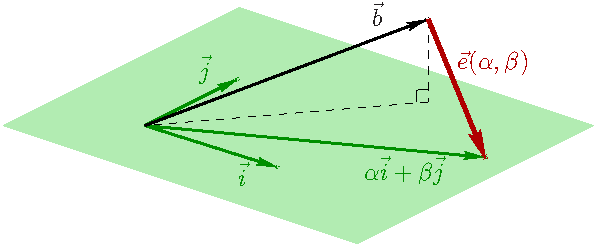
\includegraphics[width=.6\linewidth]{../manuscript/img/error.pdf}
\end{center}
\end{frame}

\begin{frame}{Back to the linear regression}
\begin{minipage}{.5\linewidth}
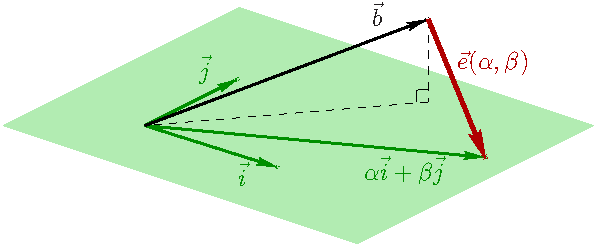
\includegraphics[width=\linewidth]{../manuscript/img/error.pdf}
\end{minipage}
\pause
\quad
\begin{minipage}{.45\linewidth}
The $\|\vec{e}(\unknown{\alpha}, \unknown{\beta})\|$ is minimized when $\vec{e}(\unknown{\alpha}, \unknown{\beta}) \perp \Span\{\known{\vec i}, \known{\vec j}\}$:
$$
\left\{
\begin{split}\known{\vec{i}}^{\,\top} \vec{e}(\unknown{\alpha}, \unknown{\beta}) &= 0\\
\known{\vec{j}}^{\,\top} \vec{e}(\unknown{\alpha}, \unknown{\beta}) &= 0
\end{split}
\right.
$$
\end{minipage}
\pause
$
\begin{bmatrix}\known{x_1} & \known{x_2} & \known{x_3} \\ 1 & 1 & 1 \end{bmatrix}
\left(\unknown{\alpha} \begin{bmatrix}\known{x_1}  \\ \known{x_2} \\ \known{x_3}  \end{bmatrix}
+\unknown{\beta} \begin{bmatrix}1 \\ 1 \\1 \end{bmatrix} -
\begin{bmatrix}\known{y_1}\\\known{y_2}\\\known{y_3}\end{bmatrix}\right) = \begin{bmatrix}0\\0\end{bmatrix}
$
\pause
\quad \qquad \qquad
$\known{A}^\top (\known{A}\unknown{x} - \known{b})= \begin{bmatrix}0\\0\end{bmatrix}$
\pause
\begin{block}{In a general case the matrix $A^\top A$ can be invertible!}
$$
A^\top Ax = A^\top b.
$$
\end{block}

\end{frame}

\begin{frame}{Some nice properties of $A^\top A$}
\begin{theorem}
$A^\top A$ is symmetric.
\end{theorem}
\pause
It is very easy to show:
$$
(A^\top A)^\top = A^\top (A^\top)^\top = A^\top A.
$$

\pause
\begin{theorem}
$A^\top A$ positive semidefinite: $\forall x\in \mathbb R^n\quad x^\top A^\top A x \geq 0.$
\end{theorem}
\pause
It follows from the fact that $x^\top A^\top A x = (A x)^\top A x > 0$.
Moreover, $A^\top A$ is positive definite in the case where $A$ has linearly independent columns (rank $A$ is equal to the number of the variables in the system).
\end{frame}

\begin{frame}{Least squares in more than two dimensions}
The same reasoning applies, here is an algebraic way to show it:
$$
\begin{aligned}
\argmin \| Ax - b \|^2 \pause &= \argmin (Ax-b)^\top (Ax-b) = \pause
 \argmin(x^\top A^\top - b^\top)(Ax-b) = \\ \pause
& = \argmin(x^\top A^\top A x - b^\top Ax - x^\top A^\top b + \underbrace{b^\top b}_{\rm const})=\\ \pause
& = \argmin(x^\top A^\top A x - 2b^\top Ax) = \pause
 \argmin(x^\top \underbrace{(A^\top A)}_{:=A'} x - 2\underbrace{(A^\top b)}_{:=b'}\phantom{}^\top x)
\end{aligned}
$$
\pause
\begin{block}{The takeaway message}
The least squares problem $\argmin \| Ax - b \|^2$  is equivalent to minimizing the quadratic function $\argmin \left(x^\top A' x - 2b'^\top x\right)$
with (in general) a symmetric positive definite matrix $A'$. This can be done by solving a linear system $A'x = b'$.
\end{block}
\end{frame}




%\fi

\section{Least squares through examples}

\begin{frame}{Linear-quadratic regulator}
Imagine a car going at $\known{v_0}=0.5$ m/s. The goal is to accelerate to $\known{v_n}=2.3$ m/s in $n=30$ s maximum.
We can control the acceleration $\unknown{u_i}$ via the gas pedal:
$$
\unknown{v_{i+1}} = \unknown{v_i} + \unknown{u_i} = \known{v_0} + \sum\limits_{j=0}^{i}\unknown{u_j} 
$$

\pause
So, we need to find $\{\unknown{u_i}\}_{i=0}^{n-1}$ that optimizes some quality criterion $J(\unknown{\vec{v}}, \unknown{\vec{u}})$:
$$
\argmin J(\unknown{\vec{v}},\unknown{\vec{u}}) \quad s.t.\quad  \unknown{v_{i+1}} = \known{v_0} + \sum\limits_{j=0}^{i}\unknown{u_j} \quad \forall i \in 0..n-1
$$

\pause
What happens if we ask for the car to reach the final speed as quickly as possible?\\
It can be written as follows:
$$
J(\unknown{\vec{v}}, \unknown{\vec{u}}) := \sum\limits_{i=1}^{n-1} (\unknown{v_i}-\known{v_n})^2 = \sum\limits_{i=1}^{n-1} \left(\sum\limits_{j=0}^{i-1}\unknown{u_j}+\known{v_0}-\known{v_n}\right)^2
$$
\end{frame}


\begin{frame}{Linear-quadratic regulator}
\begin{minipage}{.4\linewidth}
$$
J(\unknown{\vec{v}}, \unknown{\vec{u}}) := \sum\limits_{i=1}^{n-1} \left(\sum\limits_{j=0}^{i-1}\unknown{u_j}-\known{v_n}+\known{v_0}\right)^2
$$
\end{minipage}
\qquad
\begin{minipage}{.45\linewidth}
Solve in the least squares sense:\\
$
\left \{ \begin{array}{ccccl}
\unknown{u_0} &       &       &           & = \known{v_n} - \known{v_0} \\
\unknown{u_0} & + \unknown{u_1} &       &           & = \known{v_n} - \known{v_0} \\
\vdots    &       &  \ddots     &     &       \vdots      \\
\unknown{u_0} & + \unknown{u_1} & \dots & + \unknown{u_{n-1}} & = \known{v_n} - \known{v_0} \\
\end{array} \right.
$
\end{minipage}


\pause
~\\

Ouch... Quite brutal accelerations: obvious solution $u_0 = v_n-v_0$, $u_i=0 ~\forall i > 0$.
%\vspace{10pt}
%\only<2>{\inputminted[fontsize=\footnotesize,frame=single]{python}{listings/example_6.1_a.py}}
\centerline{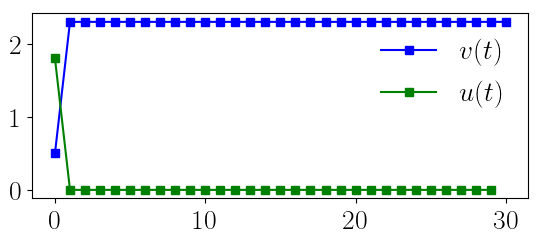
\includegraphics[width=.55\linewidth]{../manuscript/img/example_6_1_a.png}}
\end{frame}

\begin{frame}{Linear-quadratic regulator}
\begin{minipage}{.5\linewidth}
~\\
Ok, no problem, let us penalize\\ large accelerations:\\
$
J(\unknown{\vec{v}}, \unknown{\vec{u}}) := \sum\limits_{i=0}^{n-1} \unknown{u_i}^2 + \left(\sum\limits_{i=0}^{n-1} \unknown{u_i} + \known{v_0} - \known{v_n}\right)^2 
$
\end{minipage}
\qquad
\begin{minipage}{.4\linewidth}
Solve in the least squares sense:\\
$
\left \{ \begin{array}{ccccl}
\unknown{u_0} &       &       &           & = 0 \\
              & \unknown{u_1} &       &           & = 0 \\
    &       &   \ddots    &     &      \vdots       \\
              &                 &       &   \unknown{u_{n-1}} & = 0 \\
\unknown{u_0} & + \unknown{u_1} & \dots & + \unknown{u_{n-1}} & = \known{v_n} - \known{v_0} \\
\end{array} \right.
$
\end{minipage}
\pause
%\vspace{10pt}
\only<2>{\vspace{10pt}\inputminted[fontsize=\footnotesize,frame=single]{python}{listings/lqr2.py}}
\only<3>{\centerline{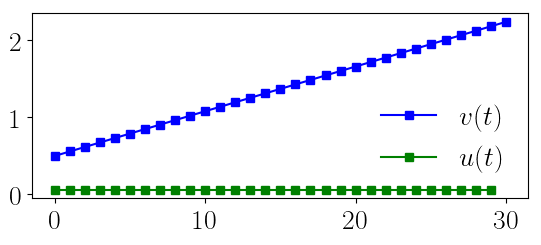
\includegraphics[width=.55\linewidth]{../manuscript/img/example_6_1_b.png}} 
Low acceleration, however the transient time becomes unacceptable.}
\end{frame}

\begin{frame}{Linear-quadratic regulator}
\begin{minipage}{.4\linewidth}
Optimize for competing goals:\\
$
J(\unknown{\vec{v}},\unknown{\vec{u}}) := \sum\limits_{i=1}^{n-1} (\unknown{v_i}-\known{v_n})^2 + \highlight{4}\sum\limits_{i=0}^{n-1} \unknown{u_i}^2 \pause = \sum\limits_{i=1}^{n-1} \left(\sum\limits_{j=0}^{i-1}\unknown{u_j}-\known{v_n}+\known{v_0}\right)^2 + \highlight{4}\sum\limits_{i=0}^{n-1} \unknown{u_i}^2
$
\textbf{N.B.} Note the tradeoff \highlight{\text{coefficients}}!
\end{minipage}
\pause
\qquad
\begin{minipage}{.45\linewidth}
\scalebox{0.85}{
$
\left \{ \begin{array}{rrrrl}
\unknown{u_0} &       &       &           & = \known{v_n} - \known{v_0} \\
\unknown{u_0} & + \unknown{u_1} &       &           & = \known{v_n} - \known{v_0} \\
\vdots    &       &   \ddots    &     &     \vdots        \\
\unknown{u_0} & + \unknown{u_1} & \dots & + \unknown{u_{n-1}} & = \known{v_n} - \known{v_0} \\
\highlight{2}\unknown{u_0} &        &       &           & = 0 \\
     &  \highlight{2}\unknown{u_1}  &       &           & = 0 \\
     &        &  \ddots     &     &  \vdots   \\
     &        &       &  \highlight{2}\unknown{u_{n-1}} & = 0 \\
\end{array} \right.
$
}
\end{minipage}
\pause
%\vspace{10pt}
\only<4>{\vspace{10pt}\inputminted[fontsize=\footnotesize,frame=single]{python}{listings/lqr3.py}}
\only<5>{\centerline{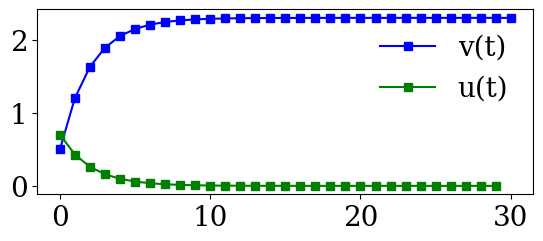
\includegraphics[width=.55\linewidth]{../manuscript/img/example_6_1_c.png}}}
\end{frame}

\begin{frame}{Linear-quadratic regulator}
\vspace{10ex}
\begin{block}{The takeaway message}
For the same problem, the same choice of variables, tweaking the objective function produces very different results. Use it!
\end{block}
\end{frame}










\begin{frame}{Poisson's equation}
\begin{minipage}{.45\linewidth}
Problem: find $\unknown{f(x)}$ defined on $x\in[0,2\pi]$ as close as possible to $g(x):=\sin x$, constrained to $\known{f(0)}=1$ and $\known{f(2\pi)} = 3$.

\vspace{5pt}
Formulate it as the Poisson's equation with Dirichlet boundary conditions:\\
$
\frac{d^2}{dx^2}\unknown{f}  = \frac{d^2}{dx^2} g \quad \text{s.t.~} \known{f(0)}=1,~\known{f(2\pi)} = 3
$
\end{minipage}
\qquad
\begin{minipage}{.4\linewidth}
\centerline{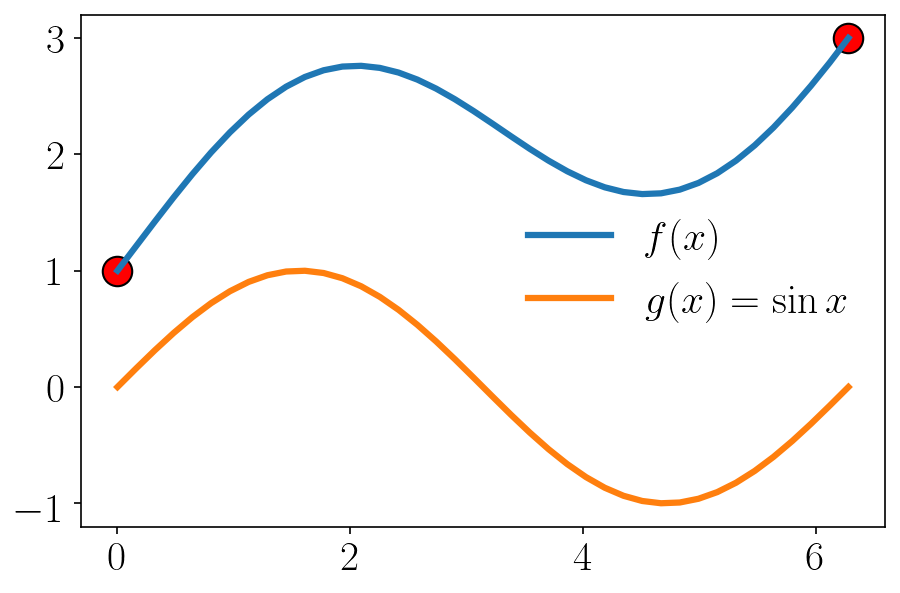
\includegraphics[width=.8\linewidth]{../manuscript/img/pie-1d.png}}
\end{minipage}

\pause

\vspace{5pt}
\textbf{Neanderthal method:}
\inputminted[fontsize=\scriptsize,frame=single]{python}{listings/poisson-1d-gauss-seidel.py}

\textbf{N.B:} extremely slow convergence for larger problems, very hard to build upon
\end{frame}


\begin{frame}{Poisson's equation}
\begin{minipage}[t]{.35\linewidth}
\strut\vspace*{-\baselineskip}\newline
\textbf{Least squares formulation:}
$$
\argmin\limits_{\unknown{f}} \int_0^{2\pi} \|\unknown{f}' - g'\|^2
$$
with $\known{f(0)}=1,~\known{f(2\pi)} = 3$
\end{minipage}
\pause
\qquad
\begin{minipage}[t]{.55\linewidth}
\strut\vspace*{-\baselineskip}\newline
\textbf{Discretization:}
$$
\left \{ \begin{array}{ccccl}
\unknown{f_1} &       &       &           & =  g_1 - g_0 + \known{f_0}  \\
-\unknown{f_1} & + \unknown{f_2} &       &           & = g_2 - g_1 \\
    &  \ddots     & \ddots      &     &       \vdots      \\
     &        &  -\unknown{f_{n-3}}     &  +\unknown{f_{n-2}}          & = g_{n-2} - g_{n-3} \\
     &        &       & - \unknown{f_{n-2}} & =  g_{n-1}-g_{n-2} -\known{f_{n-1}}
\end{array} \right.
$$
\end{minipage}

\pause
\inputminted[fontsize=\scriptsize,frame=single]{python}{listings/poisson-1d.py}
\end{frame}





\begin{frame}{Poisson image editing}
%\begin{minipage}{.66\linewidth}
\centerline{    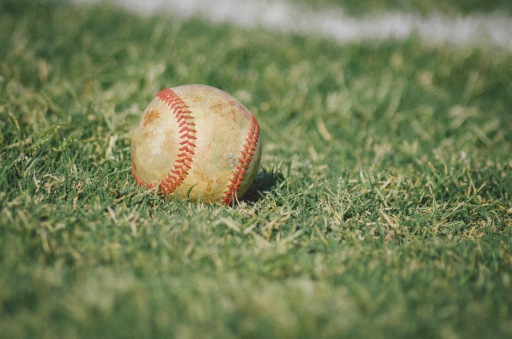
\includegraphics[width=.36\linewidth]{../manuscript/img/pie_baseball.png}~\raisebox{6.5\height}{\LARGE{+}}~
    \raisebox{0.65\height}{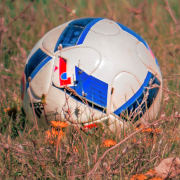
\includegraphics[width=.12\linewidth]{../manuscript/img/pie_football.png}}~\raisebox{8.5\height}{\LARGE{=}}~
    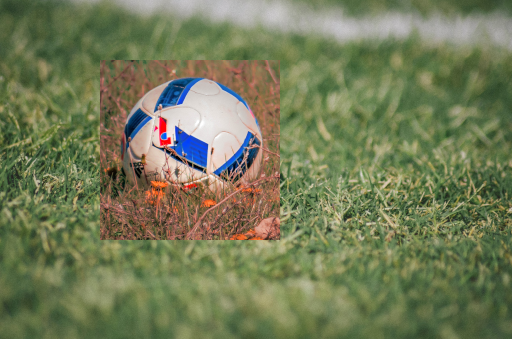
\includegraphics[width=.36\linewidth]{../manuscript/img/pie_overlay.png}}
%\end{minipage}
\pause
We can do better: solve a linear system per color channel.

\vspace{10pt}

\pause
\begin{minipage}{.12\linewidth}
Let $a$ be:\\
    
\includegraphics[width=\linewidth]{../manuscript/img/pie-baseball-red.png}
$a:\Omega\rightarrow \mathbb R$
\end{minipage}
\pause
\quad
\begin{minipage}{.12\linewidth}
Let $b$ be:\\
    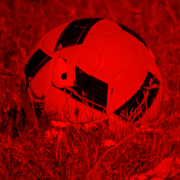
\includegraphics[width=\linewidth]{../manuscript/img/pie-football-red.png}
$b:\Omega\rightarrow \mathbb R$
\end{minipage}
\qquad
\pause
\begin{minipage}{.6\linewidth}
Solve for $\unknown{f}$ who takes its boundary conditions from $a$ and the gradients from $b$:
$$
\argmin\limits_{\unknown{f}} \int_\Omega \|\nabla \unknown{f} - \nabla b\|^2 \quad \text{with~} \unknown{f}|_{\partial\Omega} = a|_{\partial\Omega}
$$
\end{minipage}
\end{frame}

\begin{frame}{Poisson image editing}
Discretize the problem: having $w \times h$ pixels grayscale images $a$ and $b$,
we compute a $w \times h$ pixels image $\unknown{f}$, solve in the least squares sense:
$$
\left \{ \begin{array}{rll}
\unknown{f_{i+1, j}}-\unknown{f_{i,j}} & = b_{i+1, j}-b_{i,j} & \forall (i,j) \in [0 \dots w-2] \times [0\dots h-2]\\
\unknown{f_{i, j+1}}-\unknown{f_{i,j}} & = b_{i, j+1}-b_{i,j} & \forall (i,j) \in [0 \dots w-2] \times [0\dots h-2]\\
\unknown{f_{i,j}}            & = a_{i,j}            & \forall (i,j) \text{~s.t.~} i=0 \text{~or~} i=w-1 \text{~or~} j=0 \text{~or~} j=h-1
\end{array} \right.
$$

\only<1>{\textbf{N.B: sparse system solver!}}
\only<2>{
\centerline{    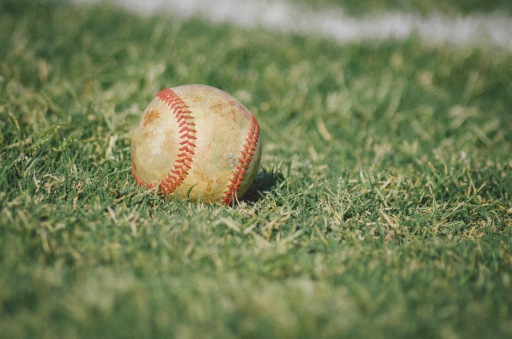
\includegraphics[width=.36\linewidth]{../manuscript/img/pie_baseball.png}~\raisebox{6.5\height}{\LARGE{+}}~
    \raisebox{0.65\height}{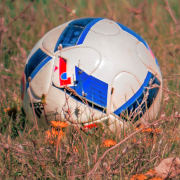
\includegraphics[width=.12\linewidth]{../manuscript/img/pie_football.png}}~\raisebox{8.5\height}{\LARGE{=}}~
    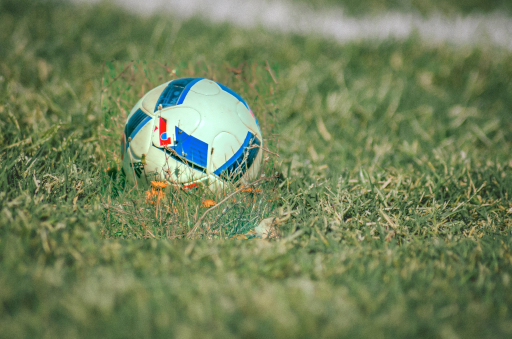
\includegraphics[width=.36\linewidth]{../manuscript/img/pie_poisson.png}}}
\end{frame}


\begin{frame}[plain,noframenumbering]
\setminted{fontsize=\tiny}
\inputminted[frame=single]{python}{listings/poisson-2d.py}
\end{frame}

\begin{frame}{Poisson's equation}
\vspace{10ex}
\begin{block}{The takeaway message}
Poisson's problem is one of the most used tools in geometry processing.\\
Know your friends!
\end{block}
\end{frame}




\begin{frame}{Caricature}
\inputminted[fontsize=\footnotesize,frame=single]{python}{listings/caricature.py}
\begin{minipage}{.55\linewidth}
    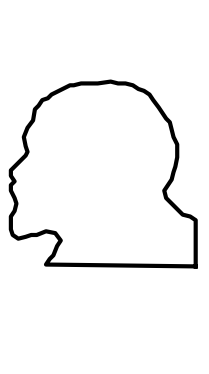
\includegraphics[height=.39\linewidth]{../manuscript/img/example_6_3_a.png}
\pause
    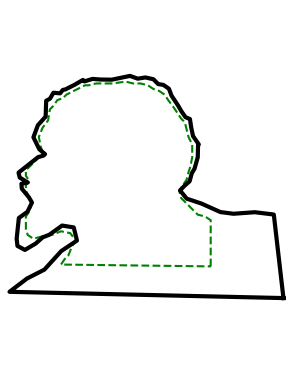
\includegraphics[height=.39\linewidth]{../manuscript/img/example_6_3_b.png}
\pause
    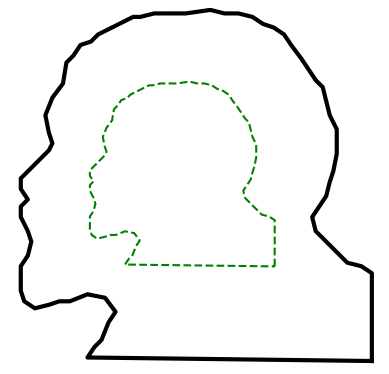
\includegraphics[height=.39\linewidth]{../manuscript/img/example_6_3_d.png}
\end{minipage}
\begin{minipage}{.44\linewidth}
Almost, but no :(
\pause
~\\

\textbf{Least squares equivalent:}\\
$\argmin\limits_{\{\unknown{x'_i}\}_{i=0}^{n-1}} \sum\limits_{\forall \text{~edge~} (i,j)} \left(\unknown{x'_j} - \unknown{x'_i} -  c\cdot\left(x_j - x_i\right)  \right)^2$\\
$x_i$ are the input coordinates and $\unknown{x_i'}$ are the unknowns (separable in x and y)
\end{minipage}
\end{frame}

\begin{frame}{Caricature}
A quick fix:\\
$\argmin\limits_{\{\unknown{x'_i}\}_{i=0}^{n-1}} ~~\sum\limits_{\forall \text{~edge~} (i,j)} \left(\unknown{x'_j} - \unknown{x'_i} -  c_0\cdot\left(x_j - x_i\right)  \right)^2 \pause \highlight{ + \sum\limits_{\forall \text{~vertex~} i} c_1^2 \left( \unknown{x'_i} - x_i \right)^2}$
\only<3>{
$$
\left \{ \begin{array}{rrrrrl}
-\unknown{x'_0}         & + \unknown{x'_1}        &                       &                           &                           & =  c_0\cdot \left( x_1 - x_0\right)  \\
                        & - \unknown{x'_1}        & +\unknown{x'_2}       &                           &                           & =  c_0 \cdot \left(x_2 - x_1\right)  \\
                        &                         &    \ddots             & \ddots                    &                           &    \vdots         \\
                        &                         &                       &   -\unknown{x'_{n-2}}     & +\unknown{x'_{n-1}}       & =  c_0 \cdot \left(x_{n-2} - x_{n-1}\right)  \\
 \unknown{x'_0}         &                         &                       &                           & -\unknown{x'_{n-1}}       & =  c_0 \cdot \left(x_{n-1} - x_0\right)  \\
c_1\cdot \unknown{x'_0} &                         &                       &                           &                           & =  c_1\cdot x_0  \\
                        & c_1\cdot \unknown{x'_1} &                       &                           &                           & =  c_1\cdot x_1  \\
                        &                         &  \multicolumn{2}{c}{                      \ddots}                    &                           & \vdots   \\
                        &                         &                       &                           &    c_1\cdot \unknown{x'_{n-1}}           & =  c_1\cdot x_{n-1}  \\
\end{array} \right.
$$
}

\begin{center}
\only<4>{
\setminted{fontsize=\tiny}
\inputminted[frame=single]{python}{listings/silhouette-better.py}
}
\only<5>{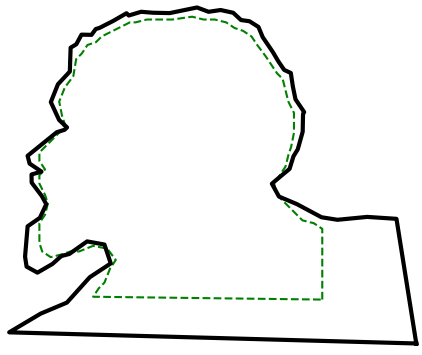
\includegraphics[width=.33\linewidth]{../manuscript/img/example_6_3_e.png}}
\only<6>{
\setminted{fontsize=\tiny}
\inputminted[frame=single]{python}{listings/caricature3d.py}
}
\only<7>{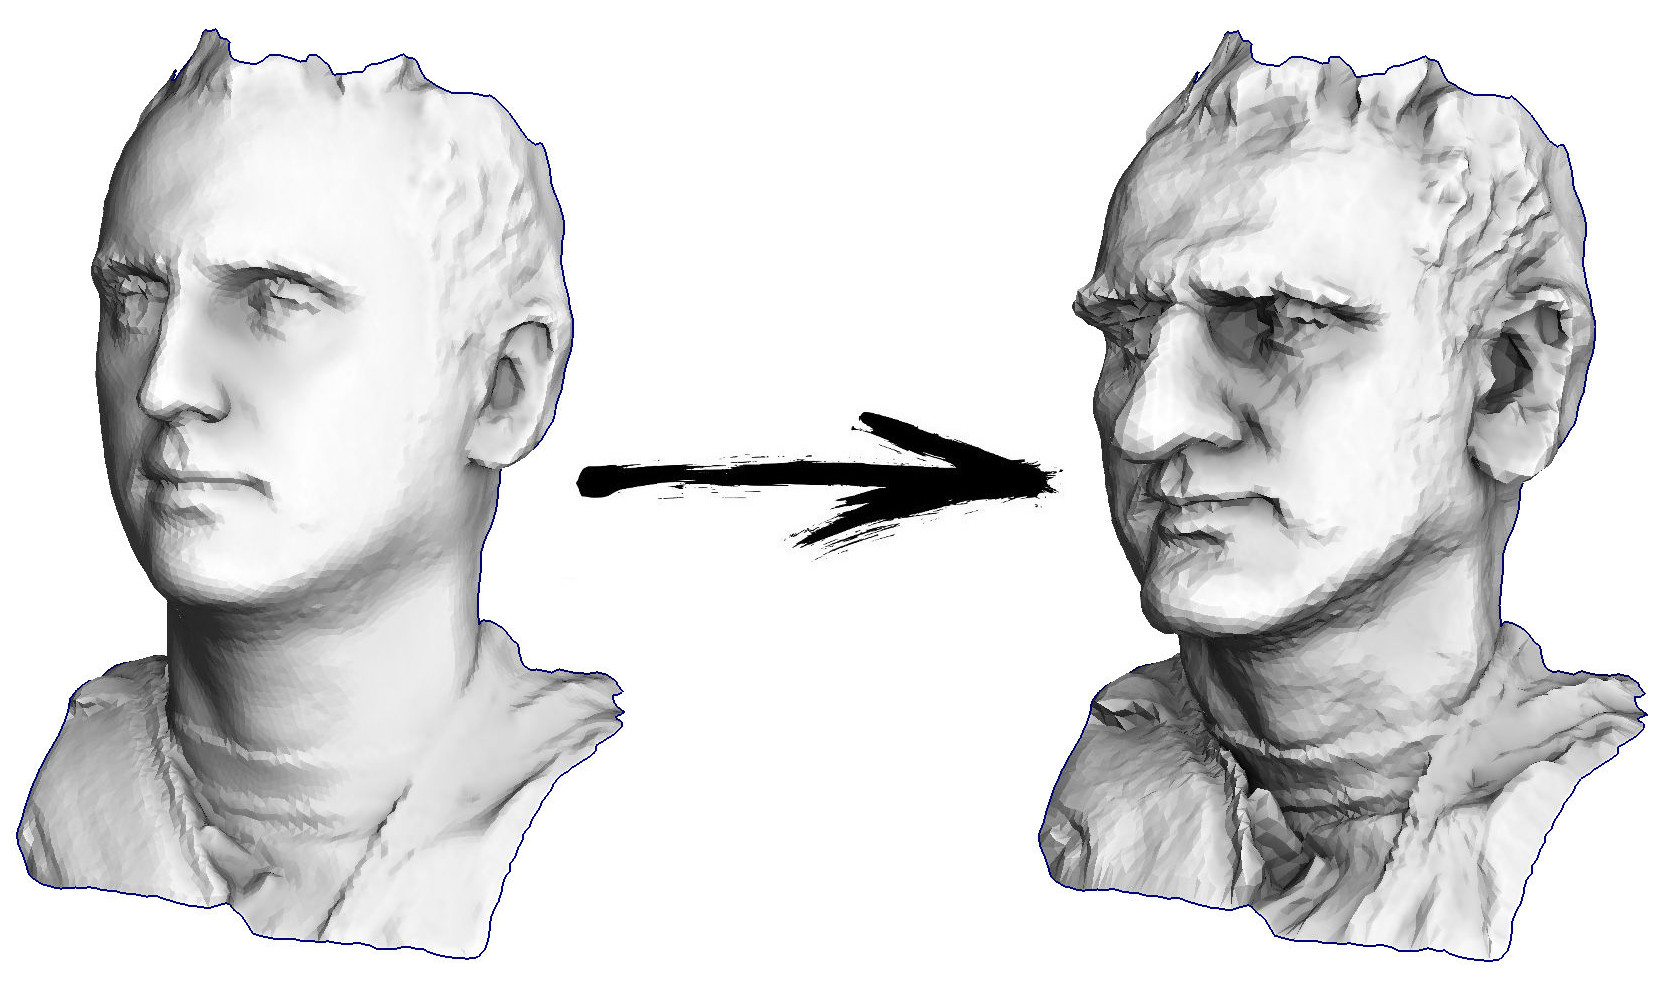
\includegraphics[width=.5\linewidth]{../manuscript/img/caricature.jpg} \\ And it works out of the box for 3d surfaces as well!}
\only<8>{
\vspace{3ex}
\begin{block}{The takeaway message}
Reformulating as a least squares problem allows for much easier tweaking.
\end{block}
}
\end{center}
\end{frame}




\begin{frame}{Cubify it!}
\begin{minipage}[t]{.4\linewidth}
\strut\vspace*{-\baselineskip}\newline
$\vec{a}_{ijk} := \argmax\limits_{\vec{a}\in \{(1,0,0), (0,1,0), (0,0,1)\}} \left|\vec{a} \cdot \vec{N}_{ijk}\right|$

\includegraphics[width=\linewidth]{../manuscript/img/cubify-flagging.jpg}
\pause
\only<3>{
\centering
\includegraphics[width=.5\linewidth]{../manuscript/img/cubify-proj.pdf}
\\
$\text{proj}_{\vec{a}} \vec{v} := \vec{v} - \frac{\vec{v}\cdot\vec{v}}{\vec{a}\cdot\vec{a}}\vec{a}$
}
\only<4>{
\vspace{-2ex}
\begin{block}{The takeaway message}
And again, the same variables,\\ but different tweaking\\ $\Rightarrow$ completely different results.
\end{block}
}
\end{minipage}
\quad
\begin{minipage}[t]{.5\linewidth}
\strut\vspace*{-\baselineskip}\newline
Let $\vec{e}_{ij}:=\vec{x}_j - \vec{x}_i$ be the input geometry, \\ and $\unknown{\vec{e}_{ij}'}:=\unknown{\vec{x}_j'} - \unknown{\vec{x}_i'}$ the unknowns.

\only<2>{
\begin{block}{Quick test}
What would be the result? \\
$\argmin\limits_{\{\unknown{\vec{x}'_i}\}_{i=0}^{n-1}} \sum\limits_{\forall \text{~edge~} ij}\left\|\unknown{\vec{e}_{ij}'} - \vec{e}_{ij}\right\|^2$
\end{block}
}
\pause
$
\arraycolsep=0pt\def\arraystretch{2.2}
\begin{array}{rll}
\argmin\limits_{\{\unknown{\vec{x}'_i}\}_{i=0}^{n-1}}~~ &\multicolumn{2}{l}{\sum\limits_{\forall \text{~edge~} ij}\left\|\unknown{\vec{e}_{ij}'} - \vec{e}_{ij}\right\|^2 +}\\
&\sum\limits_{\forall \text{~triangle~} ijk}\highlight{c}\cdot \biggl(& \left\|\unknown{\vec{e}_{ij}'} -  \text{proj}_{\vec{a}_{ijk}}  \vec{e}_{ij} \right\|^2 +\\
&&\left\|\unknown{\vec{e}_{jk}'} - \text{proj}_{\vec{a}_{ijk}}  \vec{e}_{jk} \right\|^2 +\\
&&\left\|\unknown{\vec{e}_{ki}'} - \text{proj}_{\vec{a}_{ijk}}  \vec{e}_{ki} \right\|^2\biggr)
\end{array}
$

~\\

\textbf{N.B:} still a separable problem
\end{minipage}
\pause
\end{frame}

\begin{frame}[plain,noframenumbering]
\setminted{fontsize=\scriptsize}
\inputminted[frame=single]{python}{listings/cubify.py}
\end{frame}





\begin{frame}{As-rigid-as-possible deformation}
\alt<1-2>{
Problem: compute a deformation of a mesh with several constrained vertex positions.
\centerline{ \includegraphics[width=.6\linewidth]{../manuscript/img/ARAP.jpg}}
}{}
\pause

Let $\vec{e}_{ij}:=\vec{x}_j - \vec{x}_i$ be the input geometry, and $\unknown{\vec{e}_{ij}'}:=\unknown{\vec{x}_j'} - \unknown{\vec{x}_i'}$ the unknowns.\\
Choose a subset of vertices $\mathcal I\subset [0\dots n-1]$, to have final position $\{\vec{p}_k\}_{k\in\mathcal I}$
\pause
\begin{block}{Naive solution}
$\argmin\limits_{\{\unknown{\vec{x}'_i}\}_{i=0}^{n-1}} ~\sum\limits_{\forall \text{~edge~} ij}\left\|\unknown{\vec{e}_{ij}'} - \vec{e}_{ij}\right\|^2$
subject to the constraints~ $\unknown{\vec{x}_k'} = p_k ~~ \forall k\in\mathcal I$
\end{block}

\pause
\textbf{Problem:} huge stretching near the constraints
\centerline{\includegraphics[width=0.45\linewidth]{../manuscript/img/arap-lap-a.jpg}}

\end{frame}

\begin{frame}{As-rigid-as-possible deformation}
\begin{block}{Penalize stretching: make the deformation be a rotation locally}
Introduce new variables: a rotation matrix $\unknown{R_i}$ per vertex

$\argmin\limits_{\{\unknown{\vec{x}'_i}, \unknown{R_i}\}_{i=0}^{n-1}} ~\sum\limits_{\forall \text{~edge~} ij}\left\|\unknown{\vec{e}_{ij}'} - \unknown{R_i}\times \vec{e}_{ij}\right\|^2$
\end{block}
\pause

\alt<2-5>{
\textbf{N.B:} it is a non-linear problem!

~\\

\pause
Solve alternatively for the vertex positions $\{\unknown{\vec{x}'_i}\}_{i=0}^{n-1}$ and rotations $\{\unknown{R_i}\}_{i=0}^{n-1}$:
\pause
\begin{itemize}
\item Solving for $\{\unknown{\vec{x}'_i}\}_{i=0}^{n-1}$ having $\{\known{R_i}\}_{i=0}^{n-1}$ fixed is a \textbf{separable} linear problem:\\
 3 conjugate gradients calls
\pause
\item Solving for $\{\unknown{R_i}\}_{i=0}^{n-1}$ is the \textit{orthogonal Procrustes problem} (closed form solution):
let $U_i\Sigma_i V_i^\top$ be the s.v.d. of the $3\times 3$ matrix $\sum\limits_{j \text{~neighbor of } i} \known{\vec{e}'_{ij}} \vec{e}_{ij}^\top$,
then $\unknown{R_i}\leftarrow U_i V_i^\top$
\end{itemize}
\pause
}{
\only<6>{\centerline{\includegraphics[width=0.45\linewidth]{../manuscript/img/arap-lap-a.jpg} \includegraphics[width=0.45\linewidth]{../manuscript/img/arap-lap-b.jpg}}}
\only<7>{
\vspace{4ex}
\begin{block}{The takeaway message}
Many nonlinear problems can be solved as a series of linear ones.
\end{block}
}
}
\end{frame}

\begin{frame}[plain,noframenumbering]
\setminted{fontsize=\tiny}
\inputminted[frame=single]{python}{listings/arap.py}
\end{frame}



\begin{frame}{Mix the coordinates: least squares conformal maps}
\includegraphics[width=\linewidth]{../manuscript/img/tex-mapping.pdf}
\pause
\begin{center}
How to create such a map?
\pause

\includegraphics[width=.1\linewidth]{../manuscript/img/idea.png}

Let us compute a conformal map!
\end{center}
\end{frame}

\begin{frame}{Mix the coordinates: least squares conformal maps}
\begin{minipage}{.32\linewidth}
\centering
Maps that preserve angles (but not distances or areas):

\includegraphics[width=.8\linewidth]{../manuscript/img/conformal.pdf}
\pause
Cauchy--Riemann condition:\\
$
\arraycolsep=0pt
 \begin{array}{rcl}
\frac{\partial u}{\partial x} =&  &\frac{\partial v}{\partial y} \\
\frac{\partial u}{\partial y} =& -&\frac{\partial v}{\partial x}
\end{array}
$
\end{minipage}
\pause
\quad
\begin{minipage}{.6\linewidth}
\begin{minipage}{.4\linewidth}
\includegraphics[width=\linewidth]{../manuscript/img/gradient-bg.png}
\end{minipage}
\begin{minipage}{.58\linewidth}
Sample tex coords at vertices: $(\unknown{u_i}, \unknown{v_i})$,
interpolate linearly inside triangles.\\
$\Rightarrow$
The gradient is \textbf{constant} across each triangle
\end{minipage}

\pause
\vspace{10pt}
Very simple formula for a gradient over a triangle:\\
\centerline{$\vec{N}_{ijk} \times (\nabla \unknown{u})_{ijk} = -\frac{1}{2 A_{ijk}} (\unknown{u_i} \vec{e}_{jk} + \unknown{u_j} \vec{e}_{ki} + \unknown{u_k} \vec{e}_{ij})$}

\pause

\vspace{10pt}
Sum failure of Cauchy--Riemann condition to hold:\\
\centerline{$
\argmin\limits_{\unknown{u}, \unknown{v}} \sum\limits_{\forall \text{~triangle~} ijk} A_{ijk} \biggl( 
(\nabla \unknown{u})_{ijk} - \vec{N}_{ijk} \times (\nabla \unknown{v})_{ijk}
\biggr)^2
$}

\vspace{10pt}
\textbf{N.B:} Beware of the zero solution!
\end{minipage}
\end{frame}

\begin{frame}{Mix the coordinates: least squares conformal maps}
\vspace{5pt}
Quick hack: pin two arbitrary vertices.

~\\

\centerline{
    \includegraphics[width=.2\linewidth]{../manuscript/img/lscm-head-mesh.jpg}
    \quad
    \includegraphics[width=.3\linewidth]{../manuscript/img/lscm-head-uv.jpg}
    \quad
    \includegraphics[width=.2\linewidth]{../manuscript/img/lscm-head-textured.jpg}
}
\end{frame}

\begin{frame}[plain,noframenumbering]
\setminted{fontsize=\tiny}
\inputminted[frame=single]{python}{listings/lscm.py}
\end{frame}


%\iffalse

\section{From least squares to neural networks}

\begin{frame}{Binary classification: a naive approach}
Learning database: $n$ real numbers and the corresponding colors (red and green).\\
\textbf{Problem:} build a classifying function $\mathbb R\rightarrow \{\text{red}, \text{green}\}$.

\pause
\centerline{\includegraphics[width=.5\linewidth]{../manuscript/img/binary-classification-problem.png}}
\pause
\includegraphics[width=.04\linewidth]{../manuscript/img/idea.png}
%\quad\raisebox{.5\height}{ 
Encode red as 0 and green as 1, compute the regression line over $\{(x_i, y_i)\}_{i=1}^n$,
$x_i\in\mathbb R$ and $y_i\in \{0,1\}$. The decision rule: if $y(x)>1/2$ then $x$ is green, otherwise it is red.
%}
\only<3>{
\centerline{\includegraphics[width=.5\linewidth]{../manuscript/img/linear-1d-a.png}}
\pause
}
\only<4>{
\setminted{fontsize=\tiny}
\inputminted[frame=single]{python}{listings/linear-1d.py}
\pause
}
\only<5>{\centerline{    \includegraphics[width=\linewidth]{../manuscript/img/linear-1d-b.png}}}
\end{frame}

\begin{frame}{Logistic growth}
\textbf{Limited ressources model:} a colony of the bacteria \textit{B. dendroides} is growing in a Petri dish.
The colony's area $a$ can be modeled as a function of time $t$:
$$a(t) = \frac{c}{1+e^{-wt - w_0}},$$
where $c$ is the carrying capacity, $w_0$ is the initial population size and $w$ is the growth rate.

\pause
\vspace{1ex}
\textbf{Problem:} recover the parameters $\unknown{c},\unknown{w_0},\unknown{w}$ of the model from an experiment:
\begin{minipage}{.45\linewidth}
\centerline{\includegraphics[width=\linewidth]{../manuscript/img/example_8_1_a.png}}
\end{minipage}
\begin{minipage}{.45\linewidth}
A series of $n$ measurements $\{(a_i, t_i)\}_{i=1}^n$.

\pause
$$
\argmin\limits_{\unknown{c},\unknown{w_0},\unknown{w}} \sum\limits_{i=1}^n (\unknown{a(\known{t_i})} - \known{a_i})^2
$$

\qquad\textbf{N.B:} nonlinear problem!
\end{minipage}
\end{frame}





\begin{frame}{Solve a nonlinear problem}
\begin{minipage}{.35\linewidth}
\includegraphics[width=10pt]{../manuscript/img/idea.png} \textbf{Transform the model!}

\vspace{1ex}
$\begin{aligned}
a(t) &= \frac{c}{1+e^{-wt - w_0}} \\ \pause
\frac{c}{a(t)-1} & = e^{-wt-w_0}  \\ \pause
\log\left(\frac{c-a(t)}{a(t)}\right) & = -wt-w_0
\end{aligned}
$
\end{minipage}
\quad
\begin{minipage}{.6\linewidth}
\only<6>{\setminted{fontsize=\scriptsize}
\inputminted[frame=single]{python}{listings/logistic-growth.py}
\pause
}
\only<7>{\centerline{\includegraphics[width=.8\linewidth]{../manuscript/img/example_8_1_b.png}}}
\end{minipage}

\pause
\vspace{1ex}
Ordinary linear regression provided that we have an estimation for $\unknown{c}$.\\
Ugly hack: $\known{c}:=\max\limits_{i\in 1\dots n} a_i + \varepsilon$

\pause
$$
\begin{pmatrix}
1 & t_1 \\
1 & t_2 \\
\vdots & \\
1 & t_n
\end{pmatrix}
\begin{pmatrix}
\unknown{w_0}\\
\unknown{w}
\end{pmatrix}
=
\begin{pmatrix}
\log\frac{a_1}{\known{c} - a_1}\\
\log\frac{a_2}{\known{c} - a_2}\\
\vdots \\
\log\frac{a_n}{\known{c} - a_n}
\end{pmatrix}
$$
\pause
\end{frame}



\begin{frame}{Solve a nonlinear problem: linearization}
Denote by $\vec{r}(\unknown{c},\unknown{w_0},\unknown{w})$ the residual between the input labels and the predictions:\\
\centerline{$\vec{r}(\unknown{c},\unknown{w_0},\unknown{w}) := (\unknown{a(\known{t_1})}-\known{a_1}, \dots ~\unknown{a(\known{t_n})}-\known{a_n})$}

\pause
\vspace{1ex}
\textbf{Our problem:} $\argmin\limits_{\unknown{c},\unknown{w_0},\unknown{w}} \|\vec{r}(\unknown{c},\unknown{w_0},\unknown{w})\|^2$
\qquad
\includegraphics[width=10pt]{../manuscript/img/idea.png} \textbf{Iterative optimization!} (Gauß–Newton)

\pause
\vspace{1ex}
Denote by $\unknown{\vec{b}}:=(\unknown{c},\unknown{w_0},\unknown{w})$ the vector of unknown parameters.\\
Start from an initial guess $\vec{b}^{(0)}$, build a sequence of approximations
$\vec{b}^{(k+1)} = \vec{b}^{(k)} + \unknown{\vec{\Delta}^{(k)}}$

\pause
\begin{minipage}{.5\linewidth}
Linearize the function $\vec{r}$ at the point $\vec{b}^{(k)}$:\\
\centerline{$\vec{r}(\vec{b}) \approx \vec{r}\left(\vec{b}^{(k)} \right) + J\vec{r}\left( \vec{b}^{(k)} \right) \cdot \left(\vec b - \vec{b}^{(k)}\right)$}

\pause
$\known{\Delta^{(k)}} \leftarrow \argmin\limits_{\unknown{\Delta^{(k)}}} \left\| J\vec{r}\left(\vec{b}^{(k)}\right) \unknown{\Delta^{(k)}} - \vec{r}\left(\vec{b}^{(k)}\right) \right\|^2$

\textbf{Good news:} ordinary linear regression
\end{minipage}
\pause
\begin{minipage}{.45\linewidth}
~\\

\centerline{\includegraphics[width=\linewidth]{../manuscript/img/example_8_1_c.png}}
\end{minipage}
\end{frame}

\begin{frame}[plain,noframenumbering]
\setminted{fontsize=\scriptsize}
\inputminted[frame=single]{python}{listings/logistic-1d.py}
\end{frame}

\begin{frame}{Back to the classification: quadratic loss function}
\centerline{\includegraphics[width=.9\linewidth]{../manuscript/img/linear-1d-b.png}}

\pause
\vspace{1ex}
\includegraphics[width=10pt]{../manuscript/img/idea.png} \textbf{Fit a sigmoid!} $1/(1+e^{-\unknown{w}x - \unknown{w_0}})$\\
Leave the same decision rule: $y(x)>1/2$ then $x$ is green, red otherwise.

\pause
\vspace{1ex}
Two parameters only, call Gauß–Newton:
\centerline{\includegraphics[width=.9\linewidth]{../manuscript/img/logistic-1d-b.png}}

\textbf{N.B:} attention to overfitting! May need to regularize the objective function.
\end{frame}

\begin{frame}{Good news, bad news}
\begin{minipage}[t]{.45\linewidth}
\strut\vspace*{-\baselineskip}\newline
\textbf{Good news:}\\ we have just trained a neural network

~\\

\centerline{\includegraphics[width=.9\linewidth]{../manuscript/img/neuron.pdf}}
\end{minipage}
\pause
\qquad
\begin{minipage}[t]{.45\linewidth}
\strut\vspace*{-\baselineskip}\newline
\textbf{Bad news:}\\ the energy is not convex :(

~\\
\centerline{\includegraphics[width=.9\linewidth]{../manuscript/img/ls-classification-energy.jpg}}
\end{minipage}
\end{frame}


%\fi

%\iffalse

\begin{frame}{Cross-entropy loss function}
As before, let two possible classes encoded as $y \in \{0,1\}$ and assume
$$
p(y=1|x,w) := \frac{1}{1+e^{-w^\top x}},
$$
where $w$ is a $(m+1)$-parameter vector and the last element of $x$ is the constant 1.\\

\pause
Fit the parameters of the sigmoid to match the data.
Up to this point nothing has changed!
\pause

\vspace{1ex}
\begin{block}{The game changer: Bernoulli's scheme}
$\log \mathcal{L}(w) = \log \prod_{i=1}^n p_i(w)^{y_i}  (1-p_i(w))^{1-y_i}$,
\quad where $p_i(w):=p(y_i=1|x_i, w)$.

\vspace{1ex}

\textbf{Problem:} $\argmax\limits_{\unknown{w}} \log\mathcal{L}(\unknown{w})$
\end{block}
Refer to the course notes for all details of the derivation.
\end{frame}


\begin{frame}{Cross-entropy loss function}
\textbf{Problem:} $\argmax\limits_{\unknown{w}} \log\mathcal{L}(\unknown{w}) \pause \quad \Leftrightarrow \quad \frac{\partial\log\mathcal L}{\partial \unknown{w}}(\unknown{w}) = \known{X}^\top (\known{y}-\unknown{p}) = 0,$
where $\known{X}:=\begin{bmatrix}\known{x_1} & \dots & \known{x_n}\end{bmatrix}^\top$, $\known{y}:=\begin{bmatrix}\known{y_1} & \dots & \known{y_n}\end{bmatrix}^\top$ and $\unknown{p}:=\begin{bmatrix}p_1(\unknown{w}) & \dots & p_n(\unknown{w})\end{bmatrix}^\top$.

\pause

\textbf{N.B:} Non-linear problem, but the Hessian matrix $\frac{\partial^2 \log \mathcal L}{\partial \unknown{w} \partial \unknown{w}^\top}$ is definite positive, \\ so the problem is \textbf{convex}!

\begin{minipage}{.45\linewidth}
\centerline{\includegraphics[width=.7\linewidth]{../manuscript/img/ls-vs-crossentropy-energies2.jpg}}
\end{minipage}
\pause
\begin{minipage}{.45\linewidth}
\centerline{\includegraphics[width=.7\linewidth]{../manuscript/img/logistic-regression-2d.png}}
\end{minipage}

\end{frame}

%\fi
\begin{frame}[plain,noframenumbering]
\setminted{fontsize=\scriptsize}
\inputminted[frame=single]{python}{listings/logistic-regression-2d.py}
\end{frame}


\begin{frame}{Nonlinear decision boundary: logistic regression}
\vspace{2ex}
\begin{minipage}[t]{.45\linewidth}
\strut\vspace*{-\baselineskip}\newline
\centering
%\textbf{Good news:}\\ we have just trained a neural network
%
%~\\
\centerline{\includegraphics[width=.5\linewidth]{../manuscript/img/linearly-separable-dataset.png}}
Linear decision boundary:
$$\frac{1}{1+e^{-\unknown{w}^\top x}} = \frac{1}{2}$$
\end{minipage}
\pause
%\qquad
\begin{minipage}[t]{.45\linewidth}
\strut\vspace*{-\baselineskip}\newline
\centering
\centerline{\includegraphics[width=.5\linewidth]{../manuscript/img/linearly-unseparable-dataset.png}}
Quadratic decision boundary:
$$\frac{1}{1+e^{-x^\top \unknown{A} x}} = \frac{1}{2} $$

But where is the fun in that...
%\textbf{Bad news:}\\ the energy is not convex :(
%
%~\\
%\centerline{\includegraphics[width=.9\linewidth]{../manuscript/img/ls-classification-energy.jpg}}
\end{minipage}
\end{frame}


\begin{frame}{Nonlinear decision boundary: 3 neurons}
\begin{minipage}[t]{.4\linewidth}
\strut\vspace*{-\baselineskip}\newline
Linear decision boundary:\\
\centerline{\includegraphics[width=.9\linewidth]{../manuscript/img/neuron2.pdf}}
$$
\argmin\limits_{\unknown{w}} \sum_{i=1}^{n} \left(\sigma\left(\unknown{w}^\top x_i\right) - y_i\right)^2,
$$
where $\sigma(x,w) := \frac{1}{1+e^{-w^\top x}}$
\end{minipage}
\hspace{.05\linewidth}
\pause
\begin{minipage}[t]{.5\linewidth}
\strut\vspace*{-\baselineskip}\newline
Nonlinear decision boundary:\\
\centerline{\includegraphics[width=\linewidth]{../manuscript/img/3neurons.pdf}}
$$
\argmin\limits_{\unknown{u}, \unknown{v}, \unknown{w}} \sum_{i=1}^{n} \left(\sigma\left(\unknown{w}^\top \unknown{x'_i}\right) - y_i\right)^2,
$$
where $x'_i :=  \begin{pmatrix} \sigma(\unknown{u}^\top x_i) &  \sigma(\unknown{v}^\top x_i) & 1\end{pmatrix}^\top$
\end{minipage}
\end{frame}


\begin{frame}[plain,noframenumbering]
\setminted{fontsize=\scriptsize}
\inputminted[frame=single]{python}{listings/neural.py}
\end{frame}


\begin{frame}{Nonlinear decision boundary: 3 neurons}
\centerline{\includegraphics[width=.9\linewidth]{../manuscript/img/3n.jpg}}
\pause
\centerline{\includegraphics[width=.38\linewidth]{../manuscript/img/neural.png}}
\end{frame}

\begin{frame}{The takeaway message}
\vspace{2ex}

Surprisingly, there are two irreconcilable camps: those for whom neural networks are the \textit{answer to everything}, and those who \textit{despise} neural networks.


\vspace{2ex}
I do not advocate for either party, my two main points are:

\vspace{2ex}
\begin{itemize}
\item neural networks are not the only machine learning tool;
\item there is no clear boundary between least squares methods and neural networks.
\end{itemize}
\end{frame}

\begin{frame}{Concluding remarks}
Linear regression is often underestimated being considered only as a sub-domain of statistics, but it is much more than that.

\vspace{2ex}

It offers a different view on programming:
\begin{itemize}
\item Traditionally, we break down complex tasks into a sequence of elementary operations that manipulate combinatorial structures (trees, graphs, meshes\dots).
\item Instead, we can describe what a good result looks like, and let numerical optimization algorithms find it for us.
\end{itemize}

\vspace{4ex}


\setbeamercolor{postit}{fg=black,bg=postit}
\begin{beamercolorbox}[sep=1em,wd=\linewidth]{postit}
\centering
\textbf{For any questions/remarks/corrections you are very welcome to contact me: dmitry.sokolov@univ-lorraine.fr}
\end{beamercolorbox}


\end{frame}

%\fi

\end{document}

